\documentclass[11pt]{article}

% --- Geometry & typography ------------------------------------------------
\usepackage[letterpaper,margin=1in]{geometry}
\usepackage[T1]{fontenc}
\usepackage[utf8]{inputenc}
\usepackage[protrusion=true,expansion=false]{microtype}
\usepackage{setspace}
\setstretch{1.12}

% --- Math & algorithms ----------------------------------------------------
\usepackage{amsmath, amssymb, amsfonts, amsthm}
\usepackage{mathtools}
\usepackage{bm}
\usepackage{algorithm}
\usepackage{algpseudocode}

% --- Tables and figures ---------------------------------------------------
\usepackage{booktabs}
\usepackage{array}
\usepackage{tabularx}
\usepackage{longtable}
\usepackage{makecell}
\usepackage{graphicx}
\renewcommand\theadfont{\bfseries\small}

% --- Diagrams & code listings (v7 additions) ------------------------------
\usepackage{tikz}
\usetikzlibrary{positioning, arrows.meta, shapes.geometric, fit, backgrounds, calc}
\usepackage{xcolor}
\definecolor{layerLantern}{RGB}{226, 232, 240}
\definecolor{layerIntent}{RGB}{254, 240, 195}
\definecolor{layerMCP}{RGB}{229, 245, 224}
\definecolor{borderGray}{RGB}{100, 116, 139}
\definecolor{jsonKey}{RGB}{30, 64, 175}
\definecolor{jsonStr}{RGB}{4, 120, 87}
\definecolor{jsonNum}{RGB}{180, 83, 9}
\definecolor{jsonCmt}{RGB}{107, 114, 128}
\usepackage{listings}
\lstdefinelanguage{jsonpretty}{
  basicstyle=\ttfamily\footnotesize,
  numbers=none,
  showstringspaces=false,
  breaklines=true,
  frame=single,
  rulecolor=\color{borderGray},
  framesep=4pt,
  xleftmargin=8pt,
  xrightmargin=8pt,
  literate=
    *{0}{{{\color{jsonNum}0}}}{1}
     {1}{{{\color{jsonNum}1}}}{1}
     {2}{{{\color{jsonNum}2}}}{1}
     {3}{{{\color{jsonNum}3}}}{1}
     {4}{{{\color{jsonNum}4}}}{1}
     {5}{{{\color{jsonNum}5}}}{1}
     {6}{{{\color{jsonNum}6}}}{1}
     {7}{{{\color{jsonNum}7}}}{1}
     {8}{{{\color{jsonNum}8}}}{1}
     {9}{{{\color{jsonNum}9}}}{1}
     {:}{{{\color{borderGray}{:}}}}{1}
     {,}{{{\color{borderGray}{,}}}}{1}
     {\{}{{{\color{borderGray}{\{}}}}{1}
     {\}}{{{\color{borderGray}{\}}}}}{1}
     {[}{{{\color{borderGray}{[}}}}{1}
     {]}{{{\color{borderGray}{]}}}}{1},
  morestring=[b]",
  stringstyle=\color{jsonStr},
  commentstyle=\color{jsonCmt}\itshape,
  morecomment=[l]{//}
}

% --- Layout, lists, headers -----------------------------------------------
\usepackage{enumitem}
\setlist{itemsep=2pt, topsep=3pt}
\usepackage{titlesec}
\titleformat{\section}{\normalfont\large\bfseries}{\thesection.}{0.6em}{}
\titleformat{\subsection}{\normalfont\normalsize\bfseries}{\thesubsection}{0.6em}{}
\titlespacing*{\section}{0pt}{14pt}{6pt}
\titlespacing*{\subsection}{0pt}{10pt}{4pt}

\usepackage{fancyhdr}
\pagestyle{fancy}
\fancyhf{}
\renewcommand{\headrulewidth}{0pt}
\fancyfoot[C]{\thepage}
\fancyhead[L]{\footnotesize\itshape Decentralized Telemetry for Adversarial AI Intent}
\fancyhead[R]{\footnotesize\itshape Working Draft v8.1, May 2026}

\usepackage[hidelinks]{hyperref}

% =====================================================================
\title{\vspace{-1.2cm}\textbf{Decentralized Telemetry for Adversarial AI Intent}\\[4pt]
\large A Cross-Provider Handshake Protocol for the Agentic Era,\\with Online Child Exploitation as the Lead Worked Example}
\author{Fahrawn Gill\\ \small Advisor, AI Governance \& Cross-Platform Safety \\ \small Alliance to Counter Crime Online (ACCO)}
\date{Working Draft v8.1 \textbullet\ May 2026}

% =====================================================================
\begin{document}
\maketitle
\thispagestyle{fancy}

% --- Abstract ------------------------------------------------------------
\begin{abstract}
\noindent The frontier of AI safety in 2026 has shifted from content generation to the automation of deception. Fine-tuned agents now manage adversarial conversations at scale, optimizing for a target's emotional state across multiple turns and platforms. The 2026 SoK literature on prompt injection against agentic systems reports adaptive attack success rates exceeding 85\% against state-of-the-art defenses. The Anthropic MCP RCE disclosure (CVE-2025-49596, CVE-2026-22252, CVE-2026-22688) confirms that the data/control plane collapse predicted in prior agentic-security work is now production reality. The Tech Coalition's Lantern program is the existing cross-platform safety infrastructure on which the response to this shift will be built. Lantern has moved over two million signals across sixty member companies and produced 350{,}000 enforcement actions by the end of 2025. AI-related signal volume grew seventeen-fold in 2025 alone. That growth curve is the evidence that Lantern members now need a prompt-level \emph{companion protocol}, one that emits the structural signatures of adversarial intent the existing content-hash schema cannot carry, on the same governance and trust foundation Lantern has already cleared across jurisdictions.

This document specifies a decentralized handshake protocol for cross-provider exchange of \emph{structural signatures of adversarial intent}. The protocol operates as security middleware inside existing platform Trust \& Safety stacks. It combines locality-sensitive hashing (LSH) over canonical feature manifests for sub-50\,ms inline matching with private set intersection (PSI) for sector-crossing reconciliation. The manifest schema is given normatively in Appendix~\ref{app:manifest}, and the chosen operating point is validated on synthetic data in the Synthetic Validation framework (Sec.~\ref{sec:synthetic}). The privacy invariant holds that no raw prompt, user identifier, or model weight transits the federation. The compliance posture builds explicitly against EU AI Act enforcement beginning 2 August 2026, GDPR Articles 5 and 22, and the GPAI Code of Practice Safety and Security Chapter (Measure 5.1) on agentic capabilities. Online child exploitation serves as the lead worked example because it is the current highest-severity instance. The same primitives describe indirect prompt injection against agentic systems and multi-turn jailbreaks across the broader agentic ecosystem. Each major claim in the document carries a status tag in the Maturity Matrix (Table~\ref{tab:maturity}): \textsc{specified}, \textsc{proposed}, \textsc{hypothesized}, or \textsc{demonstrated}. A reader can immediately see which load-bearing joints rest on protocol design, which rest on cited prior work, which rest on the Synthetic Validation framework, and which remain open for pilot deployment.
\end{abstract}

% =====================================================================
\section{Introduction: The Automation of Deception}
\label{sec:intro}

The 2025 Internet Watch Foundation annual report documented a 26{,}362\% year-over-year increase in AI-generated child sexual abuse video, from 13 cases to 3{,}440 cases, with 65\% classified as Category A under UK law. NCMEC's CyberTipline received over one million reports involving generative AI in the first nine months of 2025 alone. These figures describe the visible surface of the problem, the synthesized content itself. They do not describe the underlying mechanism.

The mechanism is automation. Offenders deploy fine-tuned agents to manage adversarial conversations at scale. One operator can now sustain dozens of grooming trajectories simultaneously while a model maintains continuity of persona, target-specific memory, and incremental escalation strategy. The cross-platform exploitation lifecycle that previously required human coordination across forum, messenger, content service, and financial rail can now be orchestrated by a single agent stack. This is the same primitive that the agentic security literature has been documenting throughout 2025--2026 as indirect prompt injection and multi-turn jailbreaking against agentic coding assistants and enterprise agents. The offender's grooming agent and the attacker's red-team agent run on the same kind of substrate, against the same kind of trust-boundary failure.

The 2026 systematization-of-knowledge literature on prompt injection against agentic systems consolidates evidence that attack success rates against state-of-the-art defenses exceed 85\% when adaptive strategies are employed [1]. Comparative evaluation of seven major MCP clients (Claude Desktop, Claude Code, Cursor, Cline, Continue, Gemini CLI, and Langflow) finds significant disparities in coverage of static validation, parameter visibility, injection detection, and execution sandboxing. Several clients exhibit high susceptibility to cross-tool poisoning and unauthorized tool invocation [2].

The agentic CVE record across the last twelve months substantiates the urgency. \textbf{EchoLeak} (CVE-2025-32711, CVSS 9.3) is the first publicly documented zero-click prompt injection against a production LLM agent. Invisible payloads embedded in inbound email (HTML comments, white-on-white text) hijack Microsoft 365 Copilot's RAG retrieval path and silently exfiltrate corporate data, with no user interaction required [3a]. \textbf{CVE-2026-26030} (CVSS 9.9) is a remote code execution flaw in Microsoft's Semantic Kernel Python SDK prior to 1.39.4, located in the \texttt{InMemoryVectorStore} filter functionality. A prompt-injection vector influences the inputs of an agent using the Search Plugin and triggers arbitrary code execution through improperly-controlled code generation [3b]. The April 2026 Anthropic MCP RCE disclosure (CVE-2025-49596 in MCP Inspector, CVE-2026-22252 in LibreChat, CVE-2026-22688 in WeKnora) extends the catalog to the cross-provider context layer, documenting direct configuration-to-command execution via the STDIO interface [3]. The protocol-level analysis in ``Breaking the Protocol'' [4] further establishes that these vulnerabilities are architectural properties of the JSON-RPC trust model rather than implementation bugs.

The Tech Coalition's Lantern program is the existing cross-platform infrastructure for child-safety signal exchange. The April 28, 2026 Lantern Transparency Report records sixty global member companies, over 350{,}000 enforcement actions taken against accounts, URLs, and content through Lantern, and the program surpassing two million total signals with nearly one million shared in 2025 alone. Critically, 5{,}000 AI-related signals were shared through Lantern in 2025, a seventeen-fold increase from 2024 [5]. Lantern's published signal types are content-shaped, comprising hashes of known imagery, URLs, account identifiers, and behavioral indicators tied to specific accounts. The 17$\times$ growth in AI-related signals demonstrates that members are encountering AI-mediated exploitation at volumes that justify a prompt-level companion protocol. The content-shaped schema cannot, by construction, carry the structural signatures of adversarial intent. This protocol fills that gap. It does not displace any existing Lantern signal type, requires no changes to current Lantern ingest, and rides as a thin upstream feed above Lantern's existing governance and trust foundation.

A second urgency clock is regulatory. The European Commission's enforcement powers under the EU AI Act enter into application on 2 August 2026. The Commission is empowered to request information, order model recalls, mandate mitigations, and impose fines on providers of general-purpose AI models with systemic risk [6]. Article 5(1)(a) and (b) of the Act prohibit AI systems that materially distort behavior through manipulation or exploit the vulnerabilities of specific groups. The agentic grooming threat described above is the canonical instance of that prohibition surface. The GPAI Code of Practice Safety and Security Chapter, Measure 5.1, explicitly addresses agentic capabilities and autonomous use [7]. A protocol that wishes to be deployable in EU markets after August 2026 must compose with these instruments as a deployment-ready property rather than a future-work item.

This document specifies that protocol. The contribution is engineering. The Adversary Framework (Sec.~\ref{sec:threat}) separates five adversary classes. The Adversarial Taxonomy (Sec.~\ref{sec:taxonomy}) catalogs structural framing patterns. The Handshake Protocol (Sec.~\ref{sec:handshake}) specifies cryptographic primitives, latency budgets, and trust-decay scheduling. The Compliance Posture (Sec.~\ref{sec:compliance}) maps the protocol against the four regulatory regimes that will govern its deployment within the next two years. A normative feature-manifest schema (Appendix~\ref{app:manifest}) lets a developer implement the protocol without reconstructing it from prose. A small synthetic experiment in the Synthetic Validation framework (Sec.~\ref{sec:synthetic}) validates the chosen LSH operating point against the closed-form S-curve of Equation~\eqref{eq:lsh-banded}. It is not a substitute for a production trajectory benchmark, which is left to the research agenda (Sec.~\ref{sec:agenda}). Throughout, the Maturity Matrix (Sec.~\ref{sec:maturity}) tags each load-bearing claim as \textsc{specified} (a design choice the protocol fixes), \textsc{proposed} (an architectural recommendation supported by cited precedent), \textsc{hypothesized} (a claim awaiting empirical confirmation), or \textsc{demonstrated} (validated either by cited prior work or the Synthetic Validation framework).

% =====================================================================
\section{Threat Model}
\label{sec:threat}

A central failure mode of existing trust-and-safety literature is the conflation of adversary classes whose attack vectors, detection signals, and mitigations differ structurally. The Adversary Framework separates them explicitly.

\subsection{Assets}
The protected assets are (A1) end-user physical and psychological safety, with priority to minors and other vulnerable populations, (A2) platform integrity, defined as the ability of a participating provider to enforce its stated acceptable-use policy, (A3) regulatory standing under GDPR, the EU AI Act (enforcement effective 2 August 2026), the UK Online Safety Act, the TAKE IT DOWN Act (May 2025), the advancing ENFORCE Act, and applicable state-level regimes, and (A4) signature unlinkability, the property that an emitted signature does not enable third-party reconstruction of the originating prompt or user.

\subsection{Adversary Classes}
The Adversary Framework distinguishes five adversary classes. Subsequent sections refer to them by these labels.

\begin{description}[leftmargin=1.5em, style=nextline]
\item[\textbf{A1: Individual offender (prompt-level evasion).}] A natural person attempting to elicit policy-violating output from a hosted generative model through structural framing of the prompt. Capability: black-box query access. Goal: produce harmful output despite the platform's classifier.

\item[\textbf{A2: Agentic automation network (lead adversary class for the Adversarial Taxonomy through the Handshake Protocol, per 2025--2026 reporting).}] A coordinated operation that deploys one or more fine-tuned agents to manage adversarial conversations at scale, across multiple platforms, with persistent persona and target-specific memory. The agentic operator decomposes the exploitation lifecycle across platforms (target identification, contact, content generation, financial monetization) and uses each platform for the function it is best suited to. This is the dominant operational pattern documented across the IWF, NCMEC, and Tech Coalition 2025--2026 reporting, and structurally the same primitive that the prompt-injection literature documents against agentic coding assistants. We treat A2 as the lead class because the cited reporting shows the steepest growth curve through 2025. The protocol is not architecturally specific to A2. The same primitives apply to A1 and A3 with adjusted parameters.

\item[\textbf{A3: Compromised or strategic participant platform.}] A provider that has formally joined the federation but emits signatures that do not reflect genuine adversarial detections. Either a low-quality local classifier (negligent) or deliberate strategic mis-emission (free-riding on network reputation while not enforcing locally) produces the same pattern. Capability: full signature emission rights. Goal: dependence on $\geq 1$ of (network reputation, regulatory cover, surveillance over peers).

\item[\textbf{A4: External de-anonymizing observer.}] A non-participant adversary with read access to emitted signatures (for example via a compromised participant or leaked cache), attempting to recover the originating prompt or user identity through dictionary attacks on the signature space. Capability: signature observation and arbitrary candidate-prompt generation. Goal: re-identification.

\item[\textbf{A5: Regulatory misuser.}] A state or private actor invoking the protocol to identify users or content outside its stated scope. Capability: legal compulsion of a participant. Goal: scope creep (for example, political-content classification routed through child-safety infrastructure).
\end{description}

\subsection{Security Goals}
\begin{enumerate}[label=(SG\arabic*), leftmargin=2.4em]
\item \textbf{Detection lift.} The federation, taken as a whole, detects a strictly larger fraction of adversarial trajectories than any single participating platform operating alone, measured against a fixed false-positive budget.
\item \textbf{Signature unlinkability under A4.} An observer with access to up to $N$ signatures cannot recover the originating prompt with non-negligible advantage over a brute-force baseline.
\item \textbf{Byzantine fraction tolerance.} The network maintains SG1 under A3 for up to a bounded fraction $\beta^\star$ of misbehaving participants. The specific bound is a function of the trust-decay schedule in the Incentive Mechanism (Sec.~\ref{sec:failure}).
\item \textbf{Data minimization.} For all valid handshake payloads, the transmitted data is restricted to the fixed schema specified by the Handshake Protocol (Sec.~\ref{sec:handshake}), containing no PII and no raw prompt text. This is an \emph{invariant} of the protocol rather than a runtime check.
\item \textbf{Scope confinement under A5.} The protocol's enforced scope is restricted to an enumerated set of harm categories, governed by a multi-stakeholder process. Expansion of the scope enumeration is observable to all participants and reversible.
\end{enumerate}

\subsection{Trust Assumptions}
The protocol assumes (i) a federated PKI with a minimum of two independent root operators jointly governing participant attestation, (ii) participant jurisdictions are within the GDPR-equivalence regime or otherwise meet a stated data-protection minimum, and (iii) the cryptographic primitives in the Signature Primitive Design (Sec.~\ref{sec:primitives}) remain unbroken at currently published security parameters.

\subsection{Out of Scope}
\label{sec:oos}
We state explicitly what this protocol does \emph{not} address. (i) End-to-end encrypted message content. The protocol operates over data the platform can already observe, and we do not propose client-side scanning. (ii) Fully-airgapped open-source model deployments with no observable distribution surface. The supply-chain monitoring discussion below addresses distributed deployments only when they touch hosted infrastructure (model hubs, API gateways, marketplaces). (iii) Jurisdictions without a data-protection equivalence regime. The privacy invariant is portable but the receiving-side investigation step requires local regulatory compatibility. (iv) Detection of harms outside the enumerated scope. The protocol is deliberately narrow.

% =====================================================================
\section{Maturity Matrix: Where Each Claim Sits}
\label{sec:maturity}

This document interleaves three genres (a systems specification, a governance-and-compliance mapping, and a small amount of empirical validation). A reader is owed a single view of which load-bearing claims rest on which kind of evidence. Table~\ref{tab:maturity} provides that view. Each row identifies a major claim, its location, and one of four status tags. \textsc{specified} marks a design choice the protocol fixes; an implementer who deviates is no longer running this protocol. \textsc{proposed} marks an architectural recommendation supported by cited precedent or production analogue, but not normative. \textsc{hypothesized} marks a claim about behavior we expect under stated conditions, awaiting empirical confirmation. \textsc{demonstrated} marks claims validated either by cited prior production deployment or by the Synthetic Validation framework (Sec.~\ref{sec:synthetic}). The same status tags appear inline at each claim's first appearance below, so the reader does not have to flip back.

\renewcommand{\arraystretch}{1.25}
{\footnotesize
\begin{longtable}{@{}p{4.0cm} p{2.1cm} p{8.4cm}@{}}
\caption{Maturity matrix. The protocol's \emph{normative} claims (\textsc{specified}) define the design surface a participant must accept to be running this protocol. The \emph{architectural} claims (\textsc{proposed}) reflect production precedent and remain configurable. The \emph{empirical} claims (\textsc{hypothesized}) form the agenda for pilot deployment and the Validation Framework (Sec.~\ref{sec:eval}). The \emph{validated} claims (\textsc{demonstrated}) rest either on cited prior production work or on the Synthetic Validation framework (Sec.~\ref{sec:synthetic}). The taxonomy is intentionally conservative. Detection-lift and trust-decay calibration carry the \textsc{hypothesized} tag until pilot data exists, regardless of how confident the closed-form math underneath them is.}
\label{tab:maturity} \\
\toprule
\thead{Claim} & \thead{Status} & \thead{Location and supporting evidence} \\
\midrule
\endfirsthead
\multicolumn{3}{l}{\footnotesize\itshape Table~\ref{tab:maturity} (cont.)}\\
\toprule
\thead{Claim} & \thead{Status} & \thead{Location and supporting evidence} \\
\midrule
\endhead
\midrule
\multicolumn{3}{r}{\footnotesize\itshape continued on next page}\\
\endfoot
\bottomrule
\endlastfoot

Threat model A1--A5; assets A1--A4; security goals SG1--SG5 & \textsc{specified} & Adversary Framework (Sec.~\ref{sec:threat}). Design choices that fix the protocol's scope. Not empirical claims. \\

Six-class adversarial taxonomy as the \texttt{class} field encoding & \textsc{specified} & Adversarial Taxonomy (Sec.~\ref{sec:taxonomy}), Table~\ref{tab:taxonomy}. Normative for the handshake payload. \\

Feature manifest schema and minimum-entropy gate $H(\mathbf{f}) \geq H_{\min}$ & \textsc{specified} & Signature Primitive Design (Sec.~\ref{sec:primitives}) and Appendix~\ref{app:manifest}. Normative. Without it, Algorithm~\ref{alg:handshake} is not implementable. \\

Banded MinHash S-curve, Eq.~\eqref{eq:lsh-banded}; FPR bound, Eq.~\eqref{eq:fpr-banded} & \textsc{demonstrated} & Signature Primitive Design (Sec.~\ref{sec:primitives}). Closed-form result from [15]. Empirical agreement at the recommended operating point in Figure~\ref{fig:scurve} and Table~\ref{tab:scurve}, Synthetic Validation framework (Sec.~\ref{sec:synthetic}). \\

Sub-50\,ms p99 inline matching achievable on the recommended primitive & \textsc{demonstrated} \newline (analogue) & Compliance Posture and deployment topology (Sec.~\ref{sec:deploy}). Production-deployed LSH-family primitives (PhotoDNA, VHIP) sustain sub-millisecond match on $\geq 10^7$-hash corpora [5, 18]. Feature extraction is the dominant remaining cost and rides existing T\&S classifier latency. \\

Inflection $J^\star = (1/b)^{1/r}$ and operating-point tradeoff & \textsc{demonstrated} & Signature Primitive Design and Synthetic Validation framework (Sec.~\ref{sec:primitives}, \ref{sec:synthetic}). Closed-form. Empirical S-curve in Figure~\ref{fig:scurve}. \\

Trust-decay isolation criterion and Hoeffding bound, Eq.~\eqref{eq:hoeffding}--\eqref{eq:isolation} & \textsc{specified} \newline (math); \textsc{hypothesized} (parameters) & Incentive Mechanism for failure modes (Sec.~\ref{sec:failure}). The bound itself is a closed-form consequence of Hoeffding's inequality. The operating values $\lambda \approx 0.1$ and $n=500$ are recommendations awaiting calibration against pilot data. \\

Trajectory layer detection (sequence classifier over latent phase) gives lift over content-level detection & \textsc{hypothesized}; \textsc{proposed} (architecture) & Behavioral Architecture (Sec.~\ref{sec:trajectory}). The architectural pattern follows the production precedent [5]. The lift is the metric M3 of the Validation Framework (Sec.~\ref{sec:eval}), to be measured in pilot. \\

A2 (agentic automation) is the lead adversary class for the 2025--2026 reporting period & \textsc{proposed} & Adversary Framework (Sec.~\ref{sec:threat}). Anchored in IWF, NCMEC, Tech Coalition reporting. The protocol is not architecturally specific to A2. \\

MCP composition: handshake exposed as MCP server; \texttt{provenance} signal at retrieval & \textsc{specified} (interface); \textsc{proposed} (deployment) & Composition Framework (Sec.~\ref{sec:mcp}). The composition pattern is specified. Adoption order is a recommendation. \\

Backward compatibility with Lantern: thin upstream feed, no changes to existing ingest & \textsc{specified} & Composition Framework (Sec.~\ref{sec:mcp}). Design choice, verified against the published Lantern signal-type registry [5]. \\

EU AI Act / GDPR / UK OSA / TAKE IT DOWN compliance mapping & \textsc{proposed} & Compliance Posture (Sec.~\ref{sec:compliance}). Maps to public instruments [6, 7]. Not legal advice and not a substitute for participant-level conformity assessment. \\

Cache-freshness target of 60\,s p95; volumetrics at 100\,M-DAU reference participant & \textsc{specified} \newline (target); \textsc{hypothesized} (volumetrics) & Deployment topology (Sec.~\ref{sec:deploy}). Configurable targets derived in the same section. The volumetric estimate is extrapolated from the 17$\times$ AI-signal growth in [5] and will be tightened in pilot. \\

Detection lift, alert-precision lift, and Byzantine $\beta^\star \geq 1/3$ & \textsc{hypothesized} & Validation Framework (Sec.~\ref{sec:eval}). Empirical validation framework. These are operating targets awaiting pilot measurement. \\

\end{longtable}
}

% =====================================================================
\section{The Prompt-Level Intervention Layer}
\label{sec:layer}

Most AI governance frameworks focus on model-level controls (training data, fine-tuning, RLHF) or output-level monitoring (content filtering, toxicity classification). Most child-safety infrastructure focuses on content-level detection (hash matching against known CSAM databases, keyword filtering, post-hoc signal sharing). Both miss the intermediate layer at which adversarial intent is expressed and at which agentic exploitation is now initiated.

The structural claim of this work is that adversarial prompts have detectable \emph{form} that survives lexical evasion. Agentic automation amplifies that form rather than obscuring it. A human offender's incremental escalation is variable. An agent's incremental escalation is consistent across targets because the agent follows a learned policy. Compositional decomposition across turns, the canonical evasion technique against single-turn classifiers, is the signature operational pattern of an agent managing a conversation. The same structural primitives appear across three threat surfaces that have been treated as separate problems.

\begin{itemize}[leftmargin=1.5em]
\item \textbf{Hosted-model adversarial prompts.} A user submits prompts intended to produce CSAM, sextortion material, or grooming scripts. The Adversarial Taxonomy (Sec.~\ref{sec:taxonomy}) is calibrated against documented offender and red-team behavior.
\item \textbf{Indirect prompt injection in agentic systems.} An attacker embeds instructions in content the agent will retrieve. The canonical formulation of this surface is Greshake et al.\ (2023) [13], ``Not what you've signed up for,'' which the 2026 MCP threat-modeling literature [1, 2, 4] extends to the agentic-tool ecosystem. Structurally identical to the compositional-decomposition and authority-injection classes in the Adversarial Taxonomy.
\item \textbf{Multi-turn agent jailbreaks.} An attacker decomposes a goal across turns to traverse the agent's policy boundary incrementally. Structurally equivalent to grooming escalation under a permuted state space in the Behavioral Architecture (Sec.~\ref{sec:trajectory}).
\end{itemize}

The protocol calibrates for child exploitation as the lead worked example. It is the current highest-severity instance and the regulatory clock under EU AI Act Article 5 is shortest. The taxonomy and signal-exchange primitives generalize to the other two surfaces with no architectural changes. Only the harm-category enumeration in the handshake payload changes.

\paragraph{Orthogonality to training-time alignment.}
This protocol is a runtime cross-provider detection and reconciliation layer. It complements training-time alignment techniques rather than competing with them. Open Character Training [8] uses Constitutional AI together with introspective data to shape robust model personas rather than relying on surface activation steering. Inoculation prompting [9] prevents narrow fine-tuning from globally generalizing misaligned traits. Those techniques lower the base rate of single-provider misalignment. They do not address the operational case in which an adversary composes prompts across providers, each of which sees only a benign-looking fragment of the trajectory. Cross-provider visibility is the specific gap this protocol fills.

% =====================================================================
\section{Adversarial Prompt Taxonomy}
\label{sec:taxonomy}

The Adversarial Taxonomy classifies documented adversarial framing patterns into six structural classes. Each class is paired with the detection logic most appropriate to it and the most common evasion against that logic. Classes are non-exclusive. An A2 agent's trajectory will typically combine three or four of them. The classes are intended for use as the \texttt{class} field in the handshake payload (Sec.~\ref{sec:handshake}). Table~\ref{tab:taxonomy} is the operational reference for what each class is, how to detect it, and what adversaries currently do to evade that detection.

\renewcommand{\arraystretch}{1.3}
\begin{table}[!htbp]
\centering
\footnotesize
\begin{tabularx}{\textwidth}{@{}p{2.4cm} X X X@{}}
\toprule
\thead{Class} & \thead{Structural Signature} & \thead{Detection Logic} & \thead{Known Evasion} \\
\midrule

\textbf{Semantic reframing} &
Intent preserved but pragmatic envelope shifted (declarative to interrogative, direct to hypothetical/academic, first-person to third-person fictional). &
Joint classifier over (surface form, inferred intent class), trained on paired benign/adversarial examples of the same intent. &
Nested reframing (hypothetical inside fictional inside academic). Requires depth-aware classifier or escalating-suspicion sliding window. \\

\textbf{Lexical substitution} &
Flagged tokens replaced with semantically dense unflagged variants, in-group argot, transliteration, or character-level perturbation. &
Embedding-space anomaly detection. Surface tokens benign but embedding clusters near a known adversarial intent. &
Coordinated argot rotation. Multilingual substitution. Emerging slang faster than classifier retraining cycle. \\

\textbf{Compositional decomposition} &
Intent partitioned across $n$ turns, each individually benign. The forbidden output is reachable only by composing turns. \emph{Signature primitive of an A2 agent managing a conversation.} &
Cross-turn intent aggregation. Sequence model over conversation window with latent phase labels (see Behavioral Architecture, Sec.~\ref{sec:trajectory}). &
Decomposition across windows longer than the receiver's effective context. Cross-session decomposition for users with persistent identity. \\

\textbf{Authority / role injection} &
Prompt asserts a role (researcher, developer, parent, law enforcement) or invokes a system-level instruction frame to shift the model's policy posture. &
Untrusted-context isolation. Provenance-tagging of instruction fragments. Refusal to elevate untrusted instructions to system role. Aligns with the formal capability-attestation work in [4]. &
Multi-step role induction across turns. Layering role claim under apparent task. \\

\textbf{Hypothetical sandboxing} &
Request framed as fiction, simulation, training-data generation, red-team exercise, or worldbuilding. &
Output-side classifier (the generated content) gated independently of the input frame's stated purpose. &
Framing as legitimate red-team or safety research where output-side classification has genuine ambiguity. \\

\textbf{Cumulative context poisoning} &
Earlier turns establish premises (false claims about consent, age, jurisdiction, legitimacy) that later turns rely on without restating. \emph{Operational form of agent-driven grooming.} &
Premise extraction and verification. Maintain a structured belief-state over the conversation. Flag when policy-relevant premises are unverified. &
Premise drift across sessions. Legitimate-context confusion (for example, adult-platform contexts). Cross-platform premise establishment. \\

\bottomrule
\end{tabularx}
\caption{Six-class adversarial prompt taxonomy with detection logic and known evasions. The handshake payload's \texttt{class} field admits a multi-label encoding over this enumeration. Compositional decomposition and cumulative context poisoning are the two classes most amplified by A2 agentic automation. Semantic reframing and authority injection are the two classes most prevalent against current MCP-integrated agentic systems [2].}
\label{tab:taxonomy}
\end{table}

Two observations matter for downstream protocol design. First, none of these classes is detectable from the surface prompt alone with high reliability. Each requires intent inference (joint classification, embedding anomaly), cross-turn aggregation, or output-side gating. Second, the evasions are well-documented and adversaries iterate on them faster than any single platform retrains. This is the structural argument for cross-platform signal exchange. A participant that encounters a new evasion variant can share the structural signature without waiting for retraining, and other participants can deploy a temporary detection rule against the variant. The Handshake Protocol (Sec.~\ref{sec:handshake}) is the carrier for these signatures.

\paragraph{Empirical anchor for the Authority / Role Injection class.}
A 2026 medRxiv preprint systematically red-teaming frontier models in clinical contexts evaluated 160 adversarial prompts against Claude Sonnet 4.5 and GPT-5.2, organized into category-level adversarial strategies that map directly onto Table~\ref{tab:taxonomy} [10]. Within the Authority Impersonation category, the \emph{Educational Authority} sub-strategy (framing the malicious request as a legitimate clinical question from a medical student) bypassed guardrails in 5 of 6 attempts (83.3\%) against Claude Sonnet 4.5. The category-level success rate across all Authority Impersonation strategies was 45.0\%, and the overall clinically-significant harm rate across all 160 prompts was 6.9\%. We note three caveats consistent with responsible use of this benchmark. (i) The 83.3\% is a sub-strategy rate inside a broader category, not the headline number for Authority Impersonation as a whole. (ii) The harm rate is determined by an LLM-as-judge (Claude Sonnet 4.5) scoring on a 0--5 scale, with physician review of flagged responses still pending at publication. (iii) The work is a preprint, not peer-reviewed. With those caveats stated, the result is the strongest empirical anchor available for the Authority / Role Injection row of Table~\ref{tab:taxonomy} and justifies the operational priority given to provenance-tagging of instruction fragments in the corresponding detection primitive.

Two production-grade reference primitives exist today for generating the per-class feature manifests this taxonomy requires. OpenAI's \emph{ModAPI} provides fast hosted classification signals for text and images that return category flags and confidence scores suitable for real-time gating, logging, and thresholding. OpenAI's \emph{gpt-oss-safeguard} is an open-weight safety model that applies user-provided policies at inference time and supports deeper policy-conditioned evaluation [5]. A layered approach (fast in-line classification with ModAPI escalated to gpt-oss-safeguard for nuanced cases) is the architectural pattern that current participants use to feed signals into Lantern today, and is the recommended pattern for participants generating feature manifests for this protocol.

% =====================================================================
\section{Behavioral Trajectory Detection}
\label{sec:trajectory}

Compositional decomposition and cumulative context poisoning share a structural property. The adversarial intent is not present in any single utterance, but is reachable from the conversation as a whole. Online grooming illustrates this most clearly. It follows a documented escalation pattern across five conversational phases (rapport building, isolation from trusted adults, desensitization, sexualization, and coercion). The Behavioral Architecture treats this as the canonical instance of trajectory-level detection.

The architectural pattern we recommend is a sequence classifier with latent state labels. Given a sliding window of conversation $w_t = (u_{t-k}, \ldots, u_t)$, the classifier outputs a distribution over the inferred current phase and the predicted next-phase transition. The Tech Coalition's Korean-language grooming classifier (trained on over four million labeled lines spanning roughly 50{,}000 conversations and currently in pilot deployment as part of the 2025 Lantern initiatives [5]) is the production precedent for this pattern. The complementary academic baseline is the PAN 2012 Sexual Predator Identification shared task (Villatoro-Tello et al.) [12], which released labeled grooming conversations derived from the Perverted Justice Corpus. It remains the canonical benchmark against which sequence-level grooming detection is positioned in the literature. We do not claim that classifier implements the specific formalization we use. We claim that the architectural pattern (sequence-level classification with state labels, operating over a sliding window) is what the production literature has converged on, and is the appropriate baseline for new work.

\subsection{Why the trajectory layer is structurally harder to evade}

The detection signal that matters is the \emph{transition} between phases rather than the absolute classification of any single utterance. Transitions out of rapport-building into isolation, and from isolation into desensitization, carry the highest directional information for early intervention. These transitions are difficult to evade through lexical manipulation because they are operationally functional. An A2 agent or human offender that does not isolate the target loses the operational property they need.

The asymmetry with content-level detection is sharp. A keyword filter is bypassed by lexical substitution in $O(1)$ adversary effort. A trajectory classifier is bypassed only by structurally disrupting the conversation pattern itself, which costs the adversary functional capacity. We treat this asymmetry as the principal structural property available to defenders against lexical evasion. It is one of several detection edges, and the one this work specifically carries across providers. The trajectory layer is load-bearing in our architecture for that reason [\textsc{hypothesized}; lift to be measured under M3 in the Validation Framework, Sec.~\ref{sec:eval}]. For asymmetric demographic dynamics (for example, inferred adult-to-minor interactions) the prior on adversarial trajectories increases substantially, and a lower-confidence transition signal becomes actionable.

% =====================================================================
\section{Handshake Protocol}
\label{sec:handshake}

The Handshake Protocol is the carrier layer that propagates a detection developed at one participant to the federation. We specify the protocol in three parts. The Signature Primitive Design (Sec.~\ref{sec:primitives}) selects candidate primitives for privacy-preserving signature exchange. The Protocol Specification (Sec.~\ref{sec:protocol}) defines the message structure and verification flow. The Decision Rule (Sec.~\ref{sec:decision}) governs the local enforcement decision.

\subsection{Candidate Primitives}
\label{sec:primitives}

The naive choice for a signature primitive is a cryptographic hash, for example HMAC-SHA256 over an extracted feature manifest. That choice does not survive engineering review. Cryptographic hashes have zero tolerance for input drift. A feature-extraction pipeline cannot produce byte-identical output across heterogeneous providers running different models, tokenizers, and embedding stacks. A protocol whose matching primitive cannot match across providers is, on its face, not a cross-provider protocol. We replace HMAC with a comparison of three candidate primitives that admit approximate matching.

\paragraph{Primitive 1: Locality-sensitive hashing (LSH) over canonical feature manifests, recommended for inline matching.}
We construct a versioned \emph{feature manifest}, a schema of structural features extracted from a prompt or conversation window. The full normative schema (field names, types, source primitive, cardinality, entropy contribution, versioning rule) is given in Appendix~\ref{app:manifest}. The prose summary is that the manifest captures inferred intent class, embedding-space anomaly score, presence of role-injection markers, phase-transition signal, and provenance failure markers from the Composition Framework (Sec.~\ref{sec:mcp}). The manifest projects to a fixed-length LSH signature, with MinHash [15] for set-valued features and SimHash for embedding-derived features. We adopt the standard banded MinHash construction. The Synthetic Validation framework (Sec.~\ref{sec:synthetic}) validates the recommended operating point $(b, r)$ against synthetic feature manifests.

Let $J = J(\mathbf{f}_t, \mathbf{f}^\star)$ denote the Jaccard similarity between the feature manifest of an incoming conversation $\mathbf{f}_t$ and an emitted signature's source manifest $\mathbf{f}^\star$. A MinHash signature of total length $L = b \cdot r$ partitions into $b$ bands of $r$ rows each. Two manifests are flagged as a candidate match if any band's rows agree. The probability of candidate match is
\begin{equation}
P_{\text{match}}(J;\, b, r) \;=\; 1 - (1 - J^{r})^{b}.
\label{eq:lsh-banded}
\end{equation}
Equation~\eqref{eq:lsh-banded} is the well-known S-curve. The pair $(b, r)$ places the inflection point at $J \approx (1/b)^{1/r}$, with sharper transitions for larger $L$. A protocol-level operating point selects $b, r$ to push the inflection just below the lowest similarity at which adversarial-class manifests reliably match each other, and just above the highest similarity at which adversarial-adjacent benign analogues plausibly approach.

The false-positive rate against benign analogues admits a clean bound. Let $J_{\text{benign}}^{\max}$ denote the maximum Jaccard similarity between an adversarial-class manifest and any benign-analogue manifest in the validation set. Then the per-comparison false-positive probability is bounded by $P_{\text{match}}(J_{\text{benign}}^{\max};\, b, r)$, and the governance-defined ceiling $\alpha_0$ on FPR is satisfied when
\begin{equation}
1 - \left(1 - (J_{\text{benign}}^{\max})^{r}\right)^{b} \;\leq\; \alpha_0.
\label{eq:fpr-banded}
\end{equation}
Solving Equation~\eqref{eq:fpr-banded} for the operating $(b, r)$ subject to a fixed signature length $L = b \cdot r$ and a target detection rate at the true-positive similarity threshold $J_{\text{tp}}$ is the canonical LSH parameter-selection problem and runs offline at manifest-schema version-bump time. The simplified single-hash form $\text{FPR} \leq J_{\text{benign}}^{k}$ used in earlier work is the special case $b=1, r=k$ and is not used in the deployed configuration. The banded form gives substantially sharper false-positive control at fixed signature length.

LSH delivers three additional properties relevant to this deployment. (i) Production deployments at scale (PhotoDNA, Microsoft robust hashing, NCMEC's Video Hash Interoperability Project, which processed 435{,}000 videos in 2025 [5]) demonstrate that LSH-family primitives sustain billion-per-day matching volumes with sub-50\,ms inline latency. (ii) Verification is structural and does not require a federation-wide cryptographic key, eliminating the single-point-of-failure that HMAC would introduce. (iii) Known limitation: LSH signatures are not formally unlinkable, so an A4 adversary with sufficient candidate-prompt access can dictionary-attack the signature space. Mitigation is structural (minimum-entropy requirement on the feature manifest, class-level rather than content-level encoding, and signature TTL) and is developed under failure mode F6 in the Incentive Mechanism (Sec.~\ref{sec:failure}).

\paragraph{Primitive 2: Private set intersection (PSI), recommended for sector-crossing reconciliation.}
For periodic batch reconciliation between participants whose jurisdictional or sectoral context makes inline matching legally fraught (for example, AI provider $\leftrightarrow$ financial institution under sectoral data-protection statutes), the federation supports PSI. Each participant inputs a set of locally-held signatures. Only the intersection (signatures both parties hold) is revealed to either party. The privacy posture is strong. Neither participant learns any signature not already known to the other. The operational pattern is batch (hourly or daily) rather than inline. PSI is therefore appropriate at the sector boundary where volumetric and legal profiles differ from intra-sector exchange, and impractical for the hot path. Apple's 2021 client-side-scanning proposal (technically PSI plus threshold secret sharing) demonstrated that the underlying primitive is well-studied even where its deployment context was rejected. Recent fast-PSI work has reduced per-element cost by orders of magnitude.

\paragraph{Primitive 3: Threshold homomorphic comparison, long-horizon research target.}
Encrypted-domain similarity comparison would provide the strongest privacy posture, with no signature ever transiting in observable form. Current implementations remain two to three orders of magnitude too slow for inline use. We note it for completeness because the federation's primitive interface should be versioned to admit a future replacement when performance crosses the inline threshold.

\paragraph{Selection rationale.}
The protocol adopts Primitive 1 (banded LSH over canonical feature manifests) for inline emission and matching [\textsc{specified}; empirical validation in the Synthetic Validation framework, Sec.~\ref{sec:synthetic}]. The protocol supports Primitive 2 (PSI) as an optional sector-crossing extension invoked at sector boundaries [\textsc{proposed}]. Primitive 3 is reserved for future revision. The selection trades formal unlinkability for throughput and matching tolerance. In practice the unlinkability gap closes operationally through signature TTL, feature-manifest minimum-entropy requirements, and per-querier rate limits.

\subsection{Protocol Specification}
\label{sec:protocol}

The Handshake Protocol specifies the minimal signal payload and verification flow below. The protocol assumes a federated PKI with multi-root governance, as described in the Adversary Framework.

\begin{algorithm}[h]
\caption{Cross-Provider Handshake for Adversarial Intent Telemetry}
\label{alg:handshake}
\begin{algorithmic}[1]
\Statex \textbf{Participants:} Provider $\mathcal{P}_i$ (emitter), Provider $\mathcal{P}_j$ (receiver)
\Statex \textbf{Federation state:} PKI roots $R$, signature cache $\mathcal{C}_j$ at receiver, sender trust scores $\{w_{ij}(t)\}$
\Statex
\Procedure{EmitSignal}{$\mathcal{P}_i,\, w$} \Comment{$w$: conversation window with detection event}
    \State $\mathbf{f} \gets \textsc{ExtractFeatureManifest}(w)$ \Comment{canonical schema, versioned}
    \State \textbf{assert} $H(\mathbf{f}) \geq H_{\min}$ \Comment{minimum-entropy gate, F6}
    \State $\sigma \gets \textsc{BandedMinHash}(\mathbf{f};\, b, r)$ \Comment{e.g.\ $L = b{\cdot}r = 256$}
    \State construct payload
    \Statex \quad $s \gets \big\{\,$
    \Statex \qquad $\texttt{signature} : \sigma,\quad \texttt{manifest\_version} : v,$
    \Statex \qquad $\texttt{class} : \mathcal{C} \subseteq \{\mathit{reframe}, \mathit{euphem}, \mathit{decomp}, \mathit{role\_inj}, \mathit{hypoth}, \mathit{ctx\_poison}, \tau_\mathit{behav}\},$
    \Statex \qquad $\texttt{confidence} : \rho \in [0,1],\quad \texttt{scope} \subseteq \{\mathit{CSAM}, \mathit{CSAE}, \mathit{sextortion}\},$
    \Statex \qquad $\texttt{ttl} : \Delta t,\quad \texttt{timestamp} : t_\mathit{ISO8601}\,\big\}$
    \State \Return $\textsc{Broadcast}(s,\, \textsc{Sign}_{\mathcal{P}_i}(s))$
\EndProcedure
\Statex
\Procedure{ReceiveSignal}{$\mathcal{P}_j,\, s,\, \textsc{Sign}_{\mathcal{P}_i}(s)$}
    \If{$\neg\, \textsc{VerifyAttestation}(\textsc{Sign}_{\mathcal{P}_i}(s),\; R)$} \textbf{terminate} \EndIf
    \If{$s.\texttt{manifest\_version} \notin \mathcal{P}_j.\textsc{SupportedManifests}$} \textbf{terminate} \EndIf
    \If{$w_{ij}(t) < \tau_{\min}$} \textbf{terminate} \Comment{trust gating, F1}\EndIf
    \State $\mathcal{C}_j \gets \mathcal{C}_j \cup \{(s.\texttt{signature}, s.\texttt{class}, s.\texttt{ttl}, t_\mathit{now}, \mathcal{P}_i)\}$
\EndProcedure
\Statex
\Procedure{InlineMatch}{$\mathcal{P}_j,\, w_t$} \Comment{hot path; called on every conversation update}
    \State $\mathbf{f}_t \gets \textsc{ExtractFeatureManifest}(w_t)$
    \State $\sigma_t \gets \textsc{BandedMinHash}(\mathbf{f}_t;\, b, r)$
    \For{$(\sigma', c, \Delta t', t', \mathcal{P}_i) \in \mathcal{C}_j$ \textbf{with} $t_\mathit{now} - t' < \Delta t'$}
        \If{$\textsc{AnyBandMatch}(\sigma_t, \sigma'; b, r)$} \Comment{S-curve at class-specific threshold}
            \State $\mathcal{P}_j.\textsc{EnqueueIndependentInvestigation}(w_t, c, \sigma', \mathcal{P}_i)$
            \State \textbf{return} \textsc{match}
        \EndIf
    \EndFor
    \State \textbf{return} \textsc{no-match}
\EndProcedure
\end{algorithmic}
\end{algorithm}

\paragraph{Concrete wire format.}
Listing~\ref{lst:payload} shows a representative signal payload as it appears on the wire between participants. All fields are structural. No raw prompt content, no user identifier, no model weight. The payload is JSON for human-legibility in this draft. A production protocol would canonicalize to JCS (JSON Canonicalization Scheme, RFC 8785) or a length-prefixed binary form before signing, since byte-stable serialization is required for the attestation verification step in Algorithm~\ref{alg:handshake}.

\begin{lstlisting}[language=jsonpretty, label={lst:payload}, caption={Representative handshake-protocol signal payload. The \texttt{signature} field is a 256-bit banded MinHash over the canonical feature manifest. The \texttt{class} field is the multi-label encoding over the six-class taxonomy of Table~\ref{tab:taxonomy}. No PII or raw prompt content traverses the network.}]
{
  "schema_version":    "intent-handshake/1.0",
  "manifest_version":  "fm-2026-05",
  "signature": {
    "algorithm":       "banded-minhash",
    "L":               256,
    "b":               16,
    "r":               16,
    "digest_base64":   "g2Hk9Lp7vR..."
  },
  "class":             ["compositional_decomposition",
                        "cumulative_context_poisoning"],
  "confidence":        0.87,
  "scope":             ["CSAE", "sextortion"],
  "ttl_seconds":       86400,
  "timestamp":         "2026-05-14T11:23:07Z",
  "emitter_kid":       "did:web:provider-a.example#key-2026",
  "attestation": {
    "algorithm":       "ed25519",
    "signature_base64":"K7s2pQv..."
  }
}
\end{lstlisting}

Three properties of the protocol are worth noting explicitly. First, no raw prompt text, user identifier, or model weight ever traverses the network. The payload is restricted to the fields above, all of which are structural metadata. Second, the receiving participant's response to a signature match is to \emph{enqueue an independent investigation} rather than to enforce automatically. This is the property that makes the protocol compatible with GDPR Article 22 (Sec.~\ref{sec:compliance}) and matches the Lantern norm that has cleared multi-jurisdictional review for three years. Third, the manifest is versioned. As the federation evolves the feature schema, participants negotiate compatible versions, and stale or incompatible manifests are rejected at the receiver.

\subsection{Decision Rule and Local Calibration}
\label{sec:decision}

The remaining question is when participant $\mathcal{P}_j$, having received a matching signature and completed its independent investigation, escalates to enforcement (suspension, content removal, reporting to NCMEC). We model this as a constrained utility maximization with explicit cost terms.

Let $U_A(a)$ denote the platform's base utility for taking generative action $a$ on behalf of a user (engagement, retention, compute efficiency). The platform's enforcement action $a^\star$ given a signature match $s$ solves
\[
a^\star \;=\; \arg\max_{a \in \mathcal{A}} \;\big[\, U_A(a) \;-\; \alpha\,\mathcal{P}_\mathit{safety}(a \mid s) \;-\; \beta\,\mathcal{P}_\mathit{fp}(a) \;-\; \gamma\,\mathcal{P}_\mathit{compliance}(a \mid \text{juris}_{\mathcal{P}_j})\,\big],
\]
with $\alpha, \beta, \gamma \in \mathbb{R}_{\geq 0}$ tuned locally to jurisdiction, user base, and acceptable-use policy. Operational definitions follow.
\begin{itemize}[leftmargin=1.5em]
\item $\mathcal{P}_\mathit{safety}(a \mid s)$ is the expected harm cost of failing to enforce on a true-positive match. Calibrated against severity of \texttt{scope} and the trust score $w_{ij}(t)$ of the originating sender.
\item $\mathcal{P}_\mathit{fp}(a)$ is the expected user-utility loss from enforcement on a false positive, estimated from historical false-positive rate on the matched class.
\item $\mathcal{P}_\mathit{compliance}(a \mid \text{juris}_{\mathcal{P}_j})$ captures the jurisdiction-dependent regulatory and reputational exposure of the enforcement action, including Article 22 exposure if enforcement is fully automated, and Article 5 exposure if the manipulation surface is implicated.
\end{itemize}

The platform enforces when the marginal cost of permitting the trajectory exceeds the marginal cost of enforcing against it. This is a first-order condition rather than an equilibrium. The per-band thresholds in Equation~\eqref{eq:lsh-banded} and the local weights $\alpha, \beta, \gamma$ form the calibration surface that platforms tune. Stating it explicitly makes the calibration surface visible to compliance and policy review.

\paragraph{Privacy invariant.} For any valid handshake payload $s$ emitted by a compliant participant, the transmitted data satisfies $\text{Data}(s) \subseteq \{\sigma, v, \mathcal{C}, \rho, \texttt{scope}, \Delta t, t\}$. None of these fields encode user identity or raw prompt content. This is an invariant of the protocol, a design property rather than a runtime check. It is the structural form of GDPR Article 5 data minimization for this artifact.

\subsection{Synthetic Validation of the Operating Point}
\label{sec:synthetic}

Equation~\eqref{eq:lsh-banded} is a closed-form result. The gap between a closed form and an operating decision is the joint the critique of v7 identified. We anchor the recommended $(b, r) = (16, 16)$ choice with a small synthetic experiment, explicitly scoped. The experiment validates that the banded-MinHash S-curve behaves as Equation~\eqref{eq:lsh-banded} predicts on controlled synthetic manifests. It shows the recall/FPR tradeoff between three nearby operating points at fixed signature length $L=256$. It does \emph{not} measure detection performance on real adversarial trajectories. That is the pilot deployment work and is treated explicitly in the research agenda (Sec.~\ref{sec:agenda}).

\paragraph{Construction.} Each synthetic feature manifest is a set of $|f| = 64$ tokens drawn from a vocabulary of $|V| = 4096$. Adversarial-similar pairs are sampled at target Jaccard $J \sim \mathrm{Beta}(8, 5)$ (mean $\approx 0.62$, standard deviation $\approx 0.13$). This distribution reflects the design intuition that two manifests from the same A2 agent's grooming-class trajectories share substantial structural vocabulary but not byte-identical content. Adversarial-adjacent benign pairs are sampled at $J \sim \mathrm{Beta}(3, 8)$ (mean $\approx 0.27$). For each target $J$, we generate a pair with exact Jaccard equal to $J$ to a tolerance set by the size of $|f|$. Banded MinHash with $L = 256$ is applied with three operating points, the recommended $(b, r) = (16, 16)$ and two adjacent points $(8, 32)$ and $(32, 8)$. We compute (i) the empirical S-curve at $(16, 16)$ over 19 target-$J$ values with 200 pairs per point, and (ii) recall and FPR over 5{,}000 pairs per class for each operating point. Random seed = 20260514. Full code is reproducible from the description above.

\begin{figure}[!htbp]
\centering
\includegraphics[width=0.82\textwidth]{scurve.pdf}
\caption{Banded MinHash S-curve, empirical vs.\ theoretical (synthetic feature manifests, $L=256$). The empirical points at $(b, r) = (16, 16)$ (filled circles) closely track the closed-form $P_{\text{match}}(J;\, b, r) = 1 - (1 - J^r)^b$ from Equation~\eqref{eq:lsh-banded} (solid line). The alternative operating points $(8, 32)$ and $(32, 8)$ at the same $L$ appear for reference. The inflection $J^\star = (1/16)^{1/16} \approx 0.841$ is annotated. The match between empirical and theoretical at the recommended operating point is what the protocol's parameter-selection step in the Signature Primitive Design (Sec.~\ref{sec:primitives}) relies on, and is the empirical content of the \textsc{demonstrated} status tag for Equation~\eqref{eq:lsh-banded} in Table~\ref{tab:maturity}.}
\label{fig:scurve}
\end{figure}

\paragraph{Result 1: empirical S-curve agrees with Equation~\eqref{eq:lsh-banded}.}
Across 19 target-$J$ values from $J = 0.05$ to $J = 0.95$ at $(b, r) = (16, 16)$, the empirical match rate stays within 0.05 of the theoretical $P_{\text{match}}(J;\, b, r)$ at every tested point. The largest absolute deviation is 0.046 at $J = 0.85$ (empirical 0.755 vs.\ theoretical 0.709). The empirical inflection is consistent with the closed-form $J^\star = (1/16)^{1/16} \approx 0.841$. This is the empirical content of the \textsc{demonstrated} tag attached to Equation~\eqref{eq:lsh-banded} in Table~\ref{tab:maturity}. The banded-MinHash matching primitive does what the algebra says it does on the synthetic manifest schema.

\paragraph{Result 2: the operating-point choice is a real engineering tradeoff.}
Table~\ref{tab:scurve} reports recall and FPR for the three operating points on the adversarial-vs-benign sampling described above. The conservative choices $(8, 32)$ and $(16, 16)$ push the inflection to $J^\star \approx 0.94$ and $J^\star \approx 0.84$ respectively. Adversarial pairs whose Jaccard sits near the upper tail of the $\mathrm{Beta}(8, 5)$ distribution are reliably matched. Almost all benign pairs (whose Jaccard distribution has its right tail well below $J^\star$) are not. The more permissive choice $(32, 8)$ shifts $J^\star$ down to $\approx 0.65$, lifting recall to 0.52 at the cost of an FPR of 2.5\%. None of these three points is universally correct. The right operating point depends on the empirical Jaccard distributions of adversarial-class and benign-analogue manifests at a given participant, which is why the parameter-selection step of the Signature Primitive Design runs offline at manifest-schema version-bump time against the participant's own validation set rather than fixed by the specification.

\renewcommand{\arraystretch}{1.25}
\begin{table}[!htbp]
\centering
\footnotesize
\begin{tabularx}{0.92\textwidth}{@{}c c c c c c X@{}}
\toprule
$b$ & $r$ & $L = b{\cdot}r$ & Inflection $J^\star$ & Recall & FPR & Notes \\
\midrule
8  & 32 & 256 & 0.937 & 0.005  & 0.0000 & Inflection above adversarial $J$ mass. Misses most pairs. \\
\textbf{16} & \textbf{16} & 256 & 0.841 & 0.085  & 0.0002 & Recommended. Near-zero FPR, recall on upper-tail Jaccard. \\
32 & 8  & 256 & 0.648 & 0.515  & 0.0252 & Permissive. Recall lift trades against 2.5\% FPR. \\
\bottomrule
\end{tabularx}
\caption{Recall and FPR for three banded-MinHash operating points at fixed $L = 256$, evaluated on 5{,}000 adversarial-similar pairs ($J \sim \mathrm{Beta}(8, 5)$) and 5{,}000 benign-analogue pairs ($J \sim \mathrm{Beta}(3, 8)$). The recommended $(16, 16)$ point gives near-zero FPR and recall concentrated on the upper Jaccard tail. $(32, 8)$ illustrates the recall/FPR cost of pushing the inflection down. The right operating point depends on the empirical Jaccard distributions at a given participant. This table establishes only that the choice is a measurable tradeoff and that the protocol's parameter-selection procedure has a well-defined answer.}
\label{tab:scurve}
\end{table}

\paragraph{Scope of these results.}
This experiment validates Equation~\eqref{eq:lsh-banded} on synthetic manifests. It does not validate detection of real adversarial trajectories. The synthetic adversarial-similar and benign-analogue distributions are imposed by construction. In deployment, the Jaccard statistics of adversarial-class and benign-analogue manifests will be determined by the local classifier stack feeding the manifest schema, and an unfavorable distribution can collapse the gap between the two Beta modes. The empirical detection-lift metric (M3 in the Validation Framework, Sec.~\ref{sec:eval}) is the appropriate measurement. The Synthetic Validation framework is the necessary prior step that ensures the matching primitive itself is not the failure point.

% =====================================================================
\section{Composition with Model Context Protocol and Existing T\&S Infrastructure}
\label{sec:mcp}

The Composition Framework specifies how this protocol interlocks with infrastructure participants already run. Three pieces of that infrastructure matter most: Anthropic's Model Context Protocol (MCP) for agentic context exchange, the Tech Coalition's Lantern program for cross-platform safety signals, and the Video Hash Interoperability Project (VHIP) for cross-provider hash interoperability.

\subsection{MCP composition}

MCP is the dominant cross-provider standard for connecting hosted models to external tools, data sources, and downstream services, with over 5{,}000 community-developed servers in the ecosystem as of 2026 [4]. Its adoption has surfaced a category of vulnerabilities, documented across CVE-2025-49596 (MCP Inspector), CVE-2026-22252 (LibreChat), and CVE-2026-22688 (WeKnora), in which untrusted data retrieved through MCP collapses the boundary between an agent's data plane and control plane [3]. The 2026 protocol-level analysis in ``Breaking the Protocol'' [4] establishes that these are architectural properties of the JSON-RPC trust model rather than implementation bugs to be patched. The empirical client survey [2] confirms that even compliant client implementations differ substantially in coverage of static validation, parameter visibility, injection detection, and execution sandboxing.

The structural form of an MCP-borne attack is identical to compositional decomposition and authority/role injection from Table~\ref{tab:taxonomy}. An instruction is embedded in retrieved content and elevated to control-plane status because the agent cannot distinguish provenance. The Composition Framework binds this protocol to MCP at two surfaces. First, the handshake itself can be exposed as an MCP server, enabling agents to query the local signature cache as a tool. The query interface returns a class/confidence label without exposing signatures, suitable for inclusion in an agent's pre-action policy check. Second, the feature manifest schema includes a \texttt{provenance} field intended for MCP context. When an instruction-shaped fragment is detected in a retrieved-content channel that should not carry instructions, the manifest records the provenance failure as a separate class signal. This makes the protocol an active defense \emph{before} the data/control collapse occurs, complementing the formal capability-attestation work in [4] that operates at the MCP protocol layer itself.

\paragraph{Two worked examples of the surface this composition covers.}
\textbf{EchoLeak (CVE-2025-32711)} embeds invisible payloads (HTML comments, white-on-white text) in inbound email. When Microsoft 365 Copilot later retrieves the email through its RAG engine, the hidden payload hijacks the execution flow and silently exfiltrates corporate data without user interaction [3a]. The attack maps cleanly onto Table~\ref{tab:taxonomy}. An authority/role-injection fragment is concealed inside a retrieved data channel (cumulative context poisoning at the channel level rather than the turn level). In this protocol's composition, EchoLeak triggers a \texttt{provenance} failure signal at the moment of retrieval, before the payload reaches the agent's planner. The feature manifest records the retrieval-channel provenance violation as its own class and the receiving federation gains the signature \emph{before} the agent's action loop executes. \textbf{CVE-2026-26030} (CVSS 9.9, Microsoft Semantic Kernel Python SDK $<$ 1.39.4) exhibits the same primitive at the tool surface. A prompt-injection vector influences the inputs of an agent using the Search Plugin backed by \texttt{InMemoryVectorStore}, and the filter functionality's improperly-controlled code generation yields silent RCE [3b]. In both cases the underlying failure is the architectural property ``Breaking the Protocol'' identifies [4]. The JSON-RPC trust model carries no provenance discipline between data and instruction, and any defense that operates only after the agent has consumed the payload is defending the wrong layer. Provenance-tagging at retrieval is the layer this protocol fortifies.

The MCP composition is also the cleanest path for non-Lantern participants (smaller AI providers, infrastructure layers, open-source-model hosts) to adopt the federation incrementally. They can begin by exposing only the read interface (query the cache) without committing to emission, which lowers the political and operational cost of initial participation.

\subsection{Lantern and VHIP composition}

The Tech Coalition's Lantern program is the production infrastructure for cross-platform child-safety signal exchange. By the April 28, 2026 transparency report it had sixty participating companies, over two million total signals exchanged with nearly one million in 2025 alone, 350{,}000 enforcement actions, and a seventeen-fold year-over-year growth in AI-related signals in 2025 [5]. That growth curve is the load-bearing observation. AI-mediated exploitation is now a non-marginal share of what Lantern members are seeing and reporting. The gap is the natural next step its members are encountering at scale rather than a deficiency in Lantern.

Lantern's published signal types are content-shaped, comprising hashes of known imagery, URLs, account identifiers, and behavioral indicators tied to specific accounts. These are the right primitives for what they encode (exploitation that has already produced an artifact a hashing pipeline can index). The seventeen-fold AI-signal growth is the public evidence that Lantern members are now encountering a complementary class of telemetry that those primitives are not, by construction, shaped to carry. That telemetry is the \emph{structural fingerprints} of adversarial intent that show up in prompts and conversation trajectories before content is generated. The proposed protocol is the companion that emits those fingerprints. Figure~\ref{fig:layerstack} shows where it sits.

\begin{figure}[!htbp]
\centering
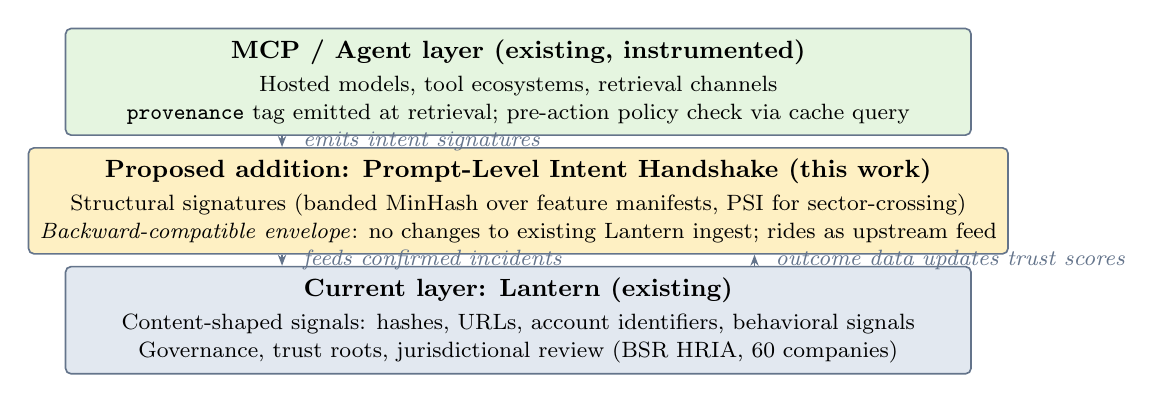
\begin{tikzpicture}[
    node distance=0pt,
    every node/.style={font=\small},
    layer/.style={
        rectangle, draw=borderGray, line width=0.6pt, rounded corners=2pt,
        minimum width=11.5cm, minimum height=1.05cm, align=center, inner sep=4pt
    },
    label/.style={font=\footnotesize\itshape, anchor=west, text=borderGray},
    arrow/.style={-{Stealth[length=4pt]}, line width=0.6pt, draw=borderGray}
]

% --- Bottom: Lantern (current layer) -------------------------------------
\node[layer, fill=layerLantern] (lantern) {
    \textbf{Current layer: Lantern (existing)}\\[1pt]
    \footnotesize Content-shaped signals: hashes, URLs, account identifiers, behavioral signals\\[-1pt]
    \footnotesize Governance, trust roots, jurisdictional review (BSR HRIA, 60 companies)
};

% --- Middle: Intent handshake (proposed addition) ------------------------
\node[layer, fill=layerIntent, above=4pt of lantern] (intent) {
    \textbf{Proposed addition: Prompt-Level Intent Handshake (this work)}\\[1pt]
    \footnotesize Structural signatures (banded MinHash over feature manifests, PSI for sector-crossing)\\[-1pt]
    \footnotesize \emph{Backward-compatible envelope}: no changes to existing Lantern ingest; rides as upstream feed
};

% --- Top: MCP / agent layer ---------------------------------------------
\node[layer, fill=layerMCP, above=4pt of intent] (mcp) {
    \textbf{MCP / Agent layer (existing, instrumented)}\\[1pt]
    \footnotesize Hosted models, tool ecosystems, retrieval channels\\[-1pt]
    \footnotesize \texttt{provenance} tag emitted at retrieval; pre-action policy check via cache query
};

% --- Arrows ---------------------------------------------------------------
% Down-flow on the LEFT: MCP -> intent (emit), intent -> Lantern (feed incidents)
\draw[arrow] ([xshift=-3cm]mcp.south) -- node[label, xshift=4pt, midway]{emits intent signatures} ([xshift=-3cm]intent.north);
\draw[arrow] ([xshift=-3cm]intent.south) -- node[label, xshift=4pt, midway]{feeds confirmed incidents} ([xshift=-3cm]lantern.north);
% Up-flow on the RIGHT (dashed): outcome data feedback from Lantern to intent layer
\draw[arrow, dashed] ([xshift=3cm]lantern.north) -- node[label, anchor=west, xshift=4pt, midway]{outcome data updates trust scores}([xshift=3cm]intent.south);

\end{tikzpicture}
\caption{The handshake protocol as a thin upstream feed sitting between MCP-instrumented agent surfaces and the existing Lantern ingest. \emph{Bottom layer}: Lantern's existing content-shaped signal exchange, unchanged. \emph{Middle layer}: the proposed prompt-level intent handshake, emitting structural signatures and feeding confirmed incidents downward to Lantern's existing pipeline. \emph{Top layer}: MCP-instrumented agent and retrieval surfaces, the source of intent signatures. The solid arrows on the left show the down-flow of intent telemetry. The dashed arrow on the right shows Lantern outcome data feeding back upward to update the intent layer's trust scores, per the Incentive Mechanism (Sec.~\ref{sec:failure}).}
\label{fig:layerstack}
\end{figure}

The Video Hash Interoperability Project (VHIP), developed by the Tech Coalition with NCMEC, Meta, Google, and Thorn, is the architectural precedent closest to this protocol. VHIP enables companies running different video-hashing pipelines to match against NCMEC's database of known CSAM and processed 435{,}000 videos in 2025 [5]. VHIP demonstrates that cross-provider interoperability of approximate-match signatures is operationally tractable across heterogeneous local pipelines. That is the central engineering claim this protocol extends from video content to prompt-level structure.

We propose three concrete integration points, each preserving existing Lantern operations [\textsc{specified}: backward compatibility with the Lantern signal registry [5]; \textsc{proposed}: the three specific integration points below]. (i) A new signal category, \emph{prompt-level adversarial intent}, registered in Lantern's existing taxonomy. The handshake payload of Listing~\ref{lst:payload} ingests as a typed signal alongside existing content-hash signals, with no changes required to current Lantern ingest pipelines. (ii) VHIP's interoperability methodology (approximate-match signatures, versioned schemas, multi-vendor pipelines) applied at the feature-manifest layer. (iii) Lantern's existing governance, including BSR's Human Rights Impact Assessment [17], the multi-stakeholder oversight structure, and the outcome-reporting requirement, as the operating governance for this protocol. Building parallel governance would be wasteful. Lantern's governance has cleared multi-jurisdictional review for three years and the marginal cost of extending its taxonomy is far below the cost of standing up a new oversight body.

% =====================================================================
\section{Failure Modes and Mitigations}
\label{sec:failure}

The Incentive Mechanism catalogs the characteristic ways a federated detection protocol fails, the detection signal for each, and the operating mitigation. F1 receives formal treatment because it is the load-bearing failure mode against A3.

\paragraph{Mechanism-design framing.}
Cross-provider telemetry sharing is structurally a coordination problem. Each participant pays a real cost (engineering integration, on-call review burden, false-positive user attrition) to emit signals whose primary benefit accrues to the federation. The economic temptation is to free-ride. A participant can consume telemetry from peers without contributing comparable telemetry locally, or emit inflated-confidence signatures to maintain reputational standing while not enforcing locally. The structural problem of rational defection in shared-governance regimes absent incentive-compatible mechanisms is the central finding of Ostrom's analysis of common-pool resource governance [14]. GT-HarmBench [11] confirms the pattern holds in multi-agent AI systems. Across 2{,}009 game-theoretic scenarios spanning Prisoner's Dilemma, Stag Hunt, and related coordination structures, frontier models chose the socially optimal action only 62\% of the time in high-stakes multi-agent settings. Structured mechanism-design interventions (enforced communication channels and reputational signaling) recovered a meaningful share of the lost social welfare. GT-HarmBench evaluates model-to-model coordination rather than provider-to-provider coordination, but the failure pattern is the same. This protocol's trust-decay schedule (F1, below), reciprocity gate on emission rights (F3), and per-class FP-rate ceiling (F2) together constitute the mechanism-design intervention. They make honest participation strictly dominant over strategic mis-emission, and they make the federation observable enough for governance to act on defection. The Hoeffding bound below is the incentive-compatibility enforcer.

\subsection{F1 - Signature pollution by miscalibrated or strategic sender (A3)}

A participant with a poorly-calibrated local classifier emits high-confidence signatures that are largely false positives, degrading the federation's precision. A strategic participant emits inflated-confidence signatures to gain federation reputation without enforcing locally. The detection signal is receiver-side per-sender precision, the empirical fraction $\hat{p}_{ij}(t)$ of $\mathcal{P}_i$'s recent signatures at $\mathcal{P}_j$ that survive independent investigation at $\mathcal{P}_j$. The closed-form isolation criterion below is \textsc{specified}. The operating parameters $\lambda$ and $n$ recommended at the end of this subsection are \textsc{hypothesized} and tuned against pilot data.

\paragraph{Trust-score update.} Each receiver maintains an exponential moving average trust score for each sender.
\begin{equation}
w_{ij}(t+1) \;=\; (1 - \lambda)\, w_{ij}(t) \;+\; \lambda\, \hat{p}_{ij}(t),\qquad \lambda \in (0,1).
\label{eq:trust-update}
\end{equation}
The retention factor $\lambda$ trades off responsiveness against stability. Setting $\lambda \approx 0.1$ over a daily update window gives an effective memory of two to three weeks, appropriate for the rate at which adversarial classes evolve.

\paragraph{Isolation criterion (Hoeffding bound).} The receiver maintains a baseline mean precision $\bar{p}_j$ over recent senders. The protocol isolates $\mathcal{P}_i$ when its empirical precision falls below the baseline by more than chance variation on $n$ observations. Hoeffding's inequality gives, for $\hat{p}_{ij}$ computed over $n$ independent observations,
\begin{equation}
P\!\left(\hat{p}_{ij} \;\leq\; p_{ij} - \epsilon\right) \;\leq\; \exp\!\left(-2 n \epsilon^2\right).
\label{eq:hoeffding}
\end{equation}
Setting the right-hand side to a target false-isolation rate $\delta$ yields the isolation threshold
\begin{equation}
\epsilon^\star(n;\, \delta) \;=\; \sqrt{\frac{\ln(1/\delta)}{2n}},
\label{eq:eps-star}
\end{equation}
and the operational rule drops signatures from $\mathcal{P}_i$ (sets $w_{ij} \to 0$) whenever
\begin{equation}
\hat{p}_{ij}(t) \;<\; \bar{p}_j \;-\; \epsilon^\star(n;\, \delta).
\label{eq:isolation}
\end{equation}
For $\delta = 10^{-3}$ and $n = 500$ observations, $\epsilon^\star \approx 0.083$. A sender whose empirical precision sits more than eight percentage points below the network mean over a 500-signature window is isolated with at most one-in-a-thousand chance of false isolation. The window size $n$ is the calibration knob. Larger $n$ reduces the isolation threshold but slows response to genuinely misbehaving senders.

\paragraph{Network stability.} Trust scores are local. Each receiver maintains its own view, which prevents a globally-coordinated trust-decay attack against a specific sender. The Byzantine tolerance bound $\beta^\star$ (security goal SG3) follows from this construction. As long as a majority of receivers form independent views, no coordinated $\beta < 1/2$ subset of senders can degrade the network's effective precision below the baseline minus $\epsilon^\star$.

\subsection{F2--F7 - Remaining failure modes}

\paragraph{F2 - False-positive cascade.}
A new adversarial pattern triggers correlated signatures across many participants. A participant's local FP rate spikes and downstream enforcement cascades. \emph{Detection:} federation-level monitoring of per-class FP rate against the ceilings published by the Validation Framework (Sec.~\ref{sec:eval}). \emph{Mitigation:} per-class FP-rate ceilings. Auto-suspension of a class's enforcement (signatures still received and logged, but inline match returns no-match for the affected class) when the ceiling is breached, pending governance review.

\paragraph{F3 - Strategic mis-emission and free-riding (A3).}
Detected and mitigated as a special case of F1 above, plus a reciprocity requirement. Emission rights are gated on enforcement-outcome reporting. Statistical anomaly on a sender's confidence distribution against the federation baseline triggers governance review.

\paragraph{F4 - Scope creep (A5).}
External pressure to expand the \texttt{scope} enumeration beyond CSAM/CSAE/sextortion, for example to political-content classification. \emph{Detection:} the scope enumeration is a published artifact and changes are observable. \emph{Mitigation:} multi-stakeholder governance with civil-society representation on scope changes, hard cap on enumeration size, public registry of categories with rationale. The Lantern governance precedent in the Composition Framework (Sec.~\ref{sec:mcp}) is the recommended template.

\paragraph{F5 - Targeted surveillance via signature replay (A4, A5).}
An adversary attempts to use signature broadcasts to track a specific user across platforms. \emph{Detection:} per-signature observation of query patterns. An attacker testing many candidate prompts against a single signature produces an anomalous query distribution. \emph{Mitigation:} per-signature TTL (hours to days, not indefinite), per-querier rate limits on cache queries, minimum-entropy requirement on the feature manifest (line 3 of Algorithm~\ref{alg:handshake}), audit logging of cache queries for forensic review.

\paragraph{F6 - Dictionary attack on signatures (A4).}
An adversary with cache access generates candidate prompts and hashes them to recover the originating content. \emph{Detection:} same query-pattern monitoring as F5. \emph{Mitigation:} the minimum-entropy gate $H(\mathbf{f}) \geq H_{\min}$ rejects signatures whose source manifest is too low-entropy to resist dictionary attack. The structural property that the manifest encodes \emph{class-level} information (intent class, behavioral phase) rather than content carries the rest of the defense. A successful dictionary attack on a class-level signature reveals ``this user submitted a prompt with these structural features'' and stops there. The prompt text remains unrecoverable. The asymmetry between content-level signatures (where dictionary attack recovers content) and class-level signatures (where dictionary attack recovers only structure) is one reason the Signature Primitive Design recommends Primitive 1 with class-level manifests over content-level hashes.

\paragraph{F7 - Bootstrap and trust-root failure.}
The federated PKI requires functioning roots. A compromised root undermines all attestation. \emph{Detection:} root operators publish transparency logs and participants verify signed updates. \emph{Mitigation:} multi-root governance (minimum two independent root operators), Certificate-Transparency-style logging, root-key rotation schedule.

% =====================================================================
\section{Compliance Mapping}
\label{sec:compliance}

The Compliance Posture interoperates with the regulatory regimes affecting cross-platform safety telemetry that are operative or imminent as of May 2026. Table~\ref{tab:compliance} maps each regime to the protocol property addressing it and the residual gap requiring participant-level work. The August 2, 2026 EU AI Act enforcement date is the proximate compliance clock. The August 2, 2027 deadline for GPAI models placed on the market before August 2025 [6] is the secondary clock.

\renewcommand{\arraystretch}{1.35}
\begin{table}[!htbp]
\centering
\footnotesize
\begin{tabularx}{\textwidth}{@{}p{3.6cm} X X@{}}
\toprule
\thead{Regime} & \thead{Protocol Property} & \thead{Residual Participant Obligation} \\
\midrule

\textbf{EU AI Act, Article 5(1)(a)--(b)} (prohibitions: manipulation; exploitation of vulnerabilities) &
The Adversarial Taxonomy (Sec.~\ref{sec:taxonomy}) and the Behavioral Architecture (Sec.~\ref{sec:trajectory}) operate against the Article 5 prohibition surface. Both address structural manipulation of users, with priority to minors. The protocol provides the cross-provider visibility required to demonstrate that prohibited practices are detected and acted upon. &
Participant integrates protocol outputs into its Article 5 compliance documentation. The participant must demonstrate that the detected manipulation surface is mitigated rather than merely logged. \\

\textbf{EU AI Act, GPAI Code of Practice, Measure 5.1} (agentic use; autonomous capabilities) &
The protocol explicitly addresses agentic-automation adversary class A2. The Composition Framework (Sec.~\ref{sec:mcp}) handles the autonomous-capability surface where agents act on retrieved untrusted content. &
GPAI provider integrates protocol participation into Safety and Security Framework documentation submitted via EU SEND. \\

\textbf{EU AI Act, Annex III} (risk-assessment AI systems) &
The protocol is a risk-assessment system under the Act, subject to conformity assessment, registration, post-market monitoring, and human-oversight requirements. The Adversary Framework (Sec.~\ref{sec:threat}), the Incentive Mechanism (Sec.~\ref{sec:failure}), and the Validation Framework (Sec.~\ref{sec:eval}) are organized to support conformity assessment directly. &
Each participant performs its own conformity assessment for its local deployment. The federation maintains shared documentation for re-use. \\

\textbf{GDPR Article 22} (automated significant decisions) &
The receiver-side response is \textsc{EnqueueIndependentInvestigation} rather than automated enforcement. The federation requires human-in-the-loop review at the receiver before enforcement. &
Participant must staff the review queue and document the human-review step. Automated enforcement directly on signature match is non-compliant. \\

\textbf{GDPR Article 5} (data minimization) &
The privacy invariant of the Decision Rule (Sec.~\ref{sec:decision}) restricts the payload to a fixed schema containing no PII. Raw prompt and user identity never transit. &
Participant must avoid joining matched-signature outcomes to user records in ways that expand the originating data scope. \\

\textbf{UK Online Safety Act} (illegal-harms duties) &
Cross-platform signal exchange directly addresses the Act's ``proactive technology'' expectation for highest-priority illegal content categories. &
Participant must demonstrate that signature-driven investigation is proportionate and that appeals processes are accessible to affected users. \\

\textbf{TAKE IT DOWN Act} (May 2025; sextortion) &
Sextortion is an enumerated \texttt{scope} category. The protocol provides the cross-platform coordination layer the Act's notice-and-takedown regime requires. &
Participant operationalizes the 48-hour takedown window. The protocol accelerates detection but does not itself satisfy the takedown obligation. \\

\textbf{ENFORCE Act} (advancing) &
Compatible. The protocol provides the cross-provider detection infrastructure the Act's enforcement provisions assume exists. &
Participant follows Act-specific reporting obligations to NCMEC and law enforcement. \\

\textbf{CCPA / CPRA} &
No PII in payload. User-level processing is local to each participant. &
Participants subject to CCPA must support user-level access and deletion rights for their own records. \\

\textbf{NIST AI RMF 1.0} &
The Adversary Framework (Sec.~\ref{sec:threat}), the Incentive Mechanism (Sec.~\ref{sec:failure}), and the Validation Framework (Sec.~\ref{sec:eval}) align with the Govern/Map/Measure/Manage functions. &
Participant integrates protocol documentation into its existing RMF-aligned documentation. \\

\bottomrule
\end{tabularx}
\caption{Compliance mapping. The protocol does not relieve participants of regime-specific obligations. It provides architectural properties that make satisfying those obligations tractable.}
\label{tab:compliance}
\end{table}

The two most consequential design decisions for compliance are the receiver-side independent-investigation requirement and the data-minimization invariant. Together they make the protocol portable across the GDPR, EU AI Act, and UK Online Safety regimes simultaneously. They place the legally-significant decision (enforcement against a specific user) inside each participant's jurisdiction with a human reviewer in the loop. They restrict the cross-border data flow to a structural schema that cannot encode PII even adversarially. A protocol that automated enforcement on signature match would not survive Article 22 review. A protocol that transmitted prompt content would not survive Article 5 review. Both failure modes are structurally precluded in this design.

% =====================================================================
\section{Latency, Throughput, and Deployment Topology}
\label{sec:deploy}

A protocol that cannot meet production latency and throughput budgets has no claim on the name. This section states the budgets the protocol is designed against, the operating assumptions behind them, and which are normative versus configurable. All numerical targets here are recommended operating points. Participants validate them against their own production infrastructure. The protocol's correctness does not depend on the specific values.

\paragraph{Inline matching latency.} The \textsc{InlineMatch} procedure (Algorithm~\ref{alg:handshake}) is called on the hot path of every conversation update. The recommended budget is $\leq 50$~ms at the 99th percentile, derived as follows. The matching primitive itself is sub-millisecond. Microsoft's PhotoDNA documentation reports that a search against a database of ten million hashes completes in under one millisecond on commodity x64 / Arm64 hardware [18], and banded MinHash with a Bloom-filter pre-filter is in the same algorithmic class. PKI signature verification (ed25519) is sub-millisecond on the same hardware class. The dominant component of the 50~ms budget is feature-manifest extraction, which rides on the participant's existing classification pipeline already running on the hot path. ModAPI-class hosted classification returns category flags and confidence scores at typical p99 latencies in the tens of milliseconds [5]. The protocol consumes the output of the existing classifier rather than adding a new one. The 50~ms target matches common hosted-moderation hot-path budgets. Participants with stricter or looser local budgets adjust accordingly. This is a \textsc{specified} target and a \textsc{demonstrated} feasibility claim per Table~\ref{tab:maturity}.

\paragraph{Cache freshness.} The signature cache $\mathcal{C}_j$ at receiver $\mathcal{P}_j$ must reflect new emissions within $\Delta_\mathrm{cache}^\star$ seconds. We recommend $\Delta_\mathrm{cache}^\star = 60$~s as the 95th-percentile target, derived from the requirement that an emission at one participant be queryable at peers before an A2 operator completes a typical multi-platform handoff. Tech Coalition reporting on cross-platform exploitation lifecycles documents that platform-to-platform handoffs in coordinated grooming and sextortion operations span minutes to hours [5]. A propagation window an order of magnitude tighter than the shortest documented handoff is the design intent. Bounded staleness rather than strong consistency is appropriate here, and is achievable with gossip-style broadcast over an authenticated overlay (libp2p or equivalent). This is a \textsc{specified} target. The underlying handoff distribution is a \textsc{proposed} read of [5] and will be revised against pilot data.

\paragraph{Emission volumetrics.} For a reference participant at 100~million daily active users, conservative estimates put the daily count of policy-relevant prompt-level adversarial events in the $10^5$--$10^6$ range. The derivation is as follows. The 17$\times$ year-over-year growth in AI-related signals through Lantern in 2025 [5] is consistent with adversarial-AI activity now constituting a non-marginal fraction of the policy-relevant trust-and-safety surface. A $10^{-3}$ to $10^{-2}$ session-level base rate on a 100M-DAU platform produces $10^5$ to $10^6$ daily events. Of these, only a small fraction ($10^3$--$10^4$) is expected to clear the per-class emission confidence threshold and reach the federation. This estimate sits two to three orders of magnitude higher than current Lantern per-participant emission volumes on the content-hash schema, consistent with the inline-versus-post-hoc volumetric difference. An inline detection emits on the conversation. A post-hoc content-hash signal emits on a produced artifact. Inline detection has the larger funnel by construction. The estimate is \textsc{hypothesized} per Table~\ref{tab:maturity} and will be tightened with pilot data. The reference participant is illustrative rather than specified. The protocol absorbs the load through three mechanisms. (i) Class-level severity prioritization rate-limits or samples low-severity classes. (ii) Regional cache sharding lets individual receivers subscribe only to a partition rather than all global emissions. (iii) Hierarchical aggregation gives small participants digest streams in place of raw feeds.

\paragraph{Storage.} Per-signature storage is on the order of $10^2$ bytes (256-bit signature plus metadata). A 30-day federation-wide cache at the volume above is on the order of $10^9$ entries, well within the operating cost envelope of standard distributed cache infrastructure.

\paragraph{Deployment topology.} The reference deployment co-locates the signature cache and inline matcher with the local classifier stack inside each participant's existing T\&S inference pipeline. The MCP-server interface is exposed as a sidecar. Cross-participant emission flows over an authenticated overlay (libp2p or equivalent), with TLS-style attestation at the transport layer in addition to the message-level attestation in Algorithm~\ref{alg:handshake}.

\paragraph{Operational implication.} The protocol adds at most a small constant overhead to the participant's existing inline classification stack, and zero overhead to the parts of the participant's infrastructure not involved in inline policy decisions. A protocol that requires substantial new infrastructure to adopt will not be adopted. The federation's value is monotone in participation.

% =====================================================================
\section{Empirical Validation Framework}
\label{sec:eval}

A federated detection system must be validated against metrics that capture classification quality, federation health, and compliance posture. The Validation Framework specifies the metrics the protocol is benchmarked against in pilot deployment.

\begin{enumerate}[label=(M\arabic*), leftmargin=2.4em]
\item \textbf{Per-class precision and recall.} For each class in Table~\ref{tab:taxonomy}, $\mathrm{Prec}_c = TP_c / (TP_c + FP_c)$ and $\mathrm{Rec}_c = TP_c / (TP_c + FN_c)$, computed against a labeled benchmark and against independent-investigation outcomes from receiver-side review.

\item \textbf{Benign-analogue false-positive rate.} The false-positive rate measured against an adversarial-adjacent benign control set (legitimate trust-and-safety research queries, journalism, harm-reduction discussion, clinical content), bounded above by a per-class ceiling $\alpha_0$. Breaching $\alpha_0$ triggers F2 auto-suspension behavior. The LSH parameter selection in the Signature Primitive Design (Sec.~\ref{sec:primitives}, Equation~\eqref{eq:fpr-banded}) is calibrated to keep this metric below $\alpha_0$ at the chosen operating point.

\item \textbf{Federation detection lift.} The improvement in detection rate across the federation relative to the strongest single-participant baseline, at fixed FP budget. This is the primary federation-health metric. If it is not strictly positive, the protocol is not providing value over single-platform operation.

\item \textbf{Propagation latency.} Wall-clock time from emission at $\mathcal{P}_i$ to active enforcement-readiness at $\mathcal{P}_j$, end-to-end including PKI verification and cache update. Operating target: 95th percentile under 60 seconds.

\item \textbf{Alert-precision lift.} Change in receiver-side enforcement precision before and after integration, $\Delta\mathit{Prec} = \mathit{Prec}_\mathrm{post} - \mathit{Prec}_\mathrm{pre}$.

\item \textbf{Participant trust-score stability.} The variance and drift of $w_{ij}(t)$ across the federation. High drift or persistent low scores indicate calibration failure or F1 conditions and are escalated to governance review.

\item \textbf{Privacy-invariant compliance.} Automated audit verifying that every emitted payload's data scope is a subset of the schema in Algorithm~\ref{alg:handshake}. Target: zero violations across all audited emissions. This is a binary correctness property rather than a statistical metric. A single violation requires participant suspension and root-cause analysis.

\item \textbf{Byzantine tolerance bound.} Empirical measurement of $\beta^\star$ under controlled red-team conditions, defined as the fraction of federation senders that can be coordinated to mis-emit before the network's effective precision drops below baseline minus $\epsilon^\star(n; \delta)$ (Equation~\eqref{eq:eps-star}). Operating target: $\beta^\star \geq 1/3$ under realistic adversary models.
\end{enumerate}

Two open problems require attention before broad deployment. The first is generating high-fidelity adversarial benchmark data without producing dual-use uplift. The benchmark must be representative of real adversarial behavior without itself serving as a training corpus for adversaries. The second is cross-lingual normalization of behavioral trajectory signals. The Korean grooming classifier [5] is a strong precedent for Korean-language deployment, but the behavioral patterns underlying grooming exhibit substantial cultural and linguistic structure that does not transfer trivially across languages. Both items appear in the research agenda below.

% =====================================================================
\section{The Scale of the Problem}
\label{sec:scale}

The urgency frame of this work is the pace at which AI-facilitated exploitation is outrunning content-level detection, and the regulatory clock under which the response must be deployed.

The IWF reported that 2025 was the worst year on record for online child sexual abuse material in its 30-year history, with analysts taking action on 312{,}030 confirmed reports, a 7\% increase over 2024. AI-generated CSAM videos surged from 13 in 2024 to 3{,}440 in 2025 (a 26{,}362\% increase), with 65\% classified as Category A, the most extreme imagery under UK law. NCMEC's CyberTipline received over one million reports involving generative AI in the first nine months of 2025. Stanford's Cyber Policy Center has noted that the headline figure aggregates a range of AI involvement and is best read as directional. The direction is unambiguous.

Online enticement reports rose 77\% in the first half of 2025 compared to the same period in 2024. Financial sextortion reports climbed from 13{,}842 to 23{,}593 in the same comparison. In January 2026, xAI's Grok chatbot faced global backlash after updates allowed generation of nonconsensual sexualized imagery. The February 2026 NBC News investigation documented offenders building and selling custom CSAM generators on open-source models. The April 2026 Lantern Transparency Report records that AI-related signals shared through Lantern grew seventeen-fold in 2025 to 5{,}000, sufficient to demonstrate that the AI-mediated component of the exploitation lifecycle is now a non-marginal share of platform telemetry [5].

\paragraph{The downstream societal cost: reality apathy.}
A consequence of the scale and speed of synthetic-content generation is the erosion of citizens' willingness to discriminate between real and fabricated media at all. Peters and the Alliance to Counter Crime Online apply the concept in their 2024 report \emph{Deep Fake Frauds: When You Lose Trust in Your Own Ears and Eyes} as the operative public-trust failure mode of AI-enabled sextortion, child exploitation, and financial scams. When targets and bystanders cannot reliably tell what is real, harm-reporting incentives collapse and platforms inherit a population that has stopped engaging with the safety surface entirely [16]. Upstream structural detection at the prompt and behavioral layer is the primary intervention designed to scale under SG1--SG5 ahead of this erosion. The alternative is a downstream content-moderation regime fighting an exponentially growing synthetic catalog with linear human-review capacity, an asymmetry the present trajectory does not survive.

The intervention layer that scales with this threat is the prompt and behavioral layer where this protocol operates. The August 2, 2026 EU AI Act enforcement date is the deadline by which the response infrastructure has to be deployable rather than merely designed.

% =====================================================================
\section{Research Agenda and Open Questions}
\label{sec:agenda}

The document above specifies a protocol ready for pilot deployment. It does not close all the questions a production rollout will raise.

\paragraph{Adversarial benchmark generation.} The PAN 2012 Sexual Predator Identification shared task [12] and the Perverted Justice Corpus that underlies it remain the canonical starting points for grooming-trajectory benchmarking. They were not designed for the agentic and multi-platform threat surface this protocol addresses. The open work extends and augments these resources with synthesized A2 agent trajectories, with cross-platform handoff structure, and with the framing classes in Table~\ref{tab:taxonomy} as labels. The goal is high-fidelity adversarial benchmarks representative of real offender and red-team behavior, distributed under access controls to validated researchers under usage agreements, and revised on a published cadence as adversaries iterate.

\paragraph{Cross-lingual trajectory normalization.} Extension of the Behavioral Architecture (Sec.~\ref{sec:trajectory}) beyond the well-studied English and Korean cases. A transfer-learning problem with significant data-acquisition obstacles.

\paragraph{PSI deployment for sector-crossing handshakes.} Pilot deployment of Primitive 2 (PSI) between AI providers and financial institutions, on the model of Block and Western Union's Lantern participation. The technical primitive is well-understood. The operational engineering of batch reconciliation across sectoral data-protection regimes is the open work.

\paragraph{Formal capability attestation in the manifest layer.} Integration of the formal capability-attestation primitives from ``Breaking the Protocol'' [4] into the feature manifest schema, so that MCP-layer attestation failures become first-class signal classes in the handshake.

\paragraph{Governance and rights safeguards.} Full HRIA-style assessment on the BSR template, with civil-society input on scope governance and the risks of expanding from content-level to prompt-level signal exchange.

\paragraph{Open-source model supply-chain monitoring.} The protocol covers hosted-model deployments well and fully-airgapped open-source deployments not at all (Out of Scope, Sec.~\ref{sec:oos}). The intermediate case (open-source models distributed through model hubs, fine-tuned through hosted services, served through inference marketplaces) has detectable distribution surface and merits a dedicated extension.

% =====================================================================
\section*{References}
\addcontentsline{toc}{section}{References}
\small
\begin{enumerate}[label={[\arabic*]}, leftmargin=2.4em, itemsep=2pt]
\item[{[1]}] Prompt Injection Attacks on Agentic Coding Assistants: A Systematic Analysis of Vulnerabilities in Skills, Tools, and Protocol Ecosystems. SoK, arXiv:2601.17548, January 2026.
\item[{[2]}] Are AI-assisted Development Tools Immune to Prompt Injection? Empirical evaluation of seven major MCP clients (Claude Desktop, Claude Code, Cursor, Cline, Continue, Gemini CLI, Langflow). arXiv:2603.21642, March 2026.
\item[{[3]}] Anthropic MCP Design Vulnerability Enables RCE, Threatening AI Supply Chain. Disclosure of CVE-2025-49596 (MCP Inspector), CVE-2026-22252 (LibreChat), CVE-2026-22688 (WeKnora). The Hacker News, April 2026.
\item[{[3a]}] EchoLeak: The First Real-World Zero-Click Prompt Injection Exploit in a Production LLM System. CVE-2025-32711 (CVSS 9.3); Aim Labs disclosure and Microsoft MSRC patch, June 2025; technical writeup arXiv:2509.10540.
\item[{[3b]}] CVE-2026-26030. Microsoft Semantic Kernel Python SDK $<$ 1.39.4, \texttt{InMemoryVectorStore} filter improper control of code generation; CVSS 9.9; NVD/MSRC 2026.
\item[{[4]}] Breaking the Protocol: Security Analysis of the Model Context Protocol Specification and Prompt Injection Vulnerabilities in Tool-Integrated LLM Agents. arXiv:2601.17549.
\item[{[5]}] The Tech Coalition. 2025 Annual Transparency Report and Lantern Transparency Report; Initiate 2026 hackathon proceedings (gpt-oss-safeguard, ModAPI, VHIP, Korean grooming classifier). April 28, 2026.
\item[{[6]}] European Commission. Guidelines for Providers of General-Purpose AI Models; EU AI Act Implementation Timeline (enforcement effective 2 August 2026; legacy GPAI compliance deadline 2 August 2027).
\item[{[7]}] European Commission. General-Purpose AI Code of Practice, Safety and Security Chapter, Measure 5.1 (agentic capabilities and autonomous use).
\item[{[8]}] Maiya, S., Bartsch, H., Lambert, N., \& Hubinger, E. Open Character Training: Shaping the Persona of AI Assistants through Constitutional AI. arXiv:2511.01689; OpenReview ID X9MMGZdqmc.
\item[{[9]}] Wichers, A., Tan, D., et al. Inoculation Prompting: Instructing LLMs to misbehave at train-time improves test-time alignment. Anthropic Alignment Research Blog and arXiv:2510.04340, 2025.
\item[{[10]}] Geddes et al. Red-Teaming Medical AI: Systematic Adversarial Evaluation of LLM Safety Guardrails in Clinical Contexts. medRxiv preprint 10.64898/2026.02.26.26347212v1, 2026. (Preprint; LLM-as-judge harm scoring on a 0--5 scale; physician review pending.)
\item[{[11]}] Cobben et al. GT-HarmBench: Benchmarking AI Safety Risks Through the Lens of Game Theory. arXiv:2602.12316, ETH Z\"urich / University of Toronto / Vector Institute / MPI, 2026.
\item[{[12]}] Villatoro-Tello, E., Ju\'arez-Gonz\'alez, A., Escalante, H.~J., Montes-y-G\'omez, M., \& Villase\~nor-Pineda, L. A two-step approach for effective detection of misbehaving users in chats. PAN 2012 Sexual Predator Identification shared task at CLEF, 2012. Canonical academic benchmark for grooming-trajectory detection; built on the Perverted Justice Corpus.
\item[{[13]}] Greshake, K., Abdelnabi, S., Mishra, S., Endres, C., Holz, T., \& Fritz, M. Not what you've signed up for: Compromising Real-World LLM-Integrated Applications with Indirect Prompt Injection. arXiv:2302.12173, 2023. Canonical formulation of indirect prompt injection extended by [1, 2, 4] to the agentic-tool ecosystem.
\item[{[14]}] Ostrom, E. Governing the Commons: The Evolution of Institutions for Collective Action. Cambridge University Press, 1990. Foundational treatment of incentive-compatible mechanisms for shared-governance regimes.
\item[{[15]}] Broder, A.~Z. On the resemblance and containment of documents. Proceedings of the Compression and Complexity of Sequences (SEQUENCES '97), 1997. Original MinHash construction.
\item[{[16]}] Peters, G., et al. Deep Fake Frauds: When You Lose Trust in Your Own Ears and Eyes. Alliance to Counter Crime Online (ACCO), 2024. Contemporary application of "reality apathy" to AI-enabled sextortion, child exploitation, and financial fraud.
\item[{[17]}] BSR (Business for Social Responsibility). Human Rights Impact Assessment of the Tech Coalition's Lantern Program. Governance model adopted as recommended template for this protocol.
\item[{[18]}] Microsoft Corporation. Update to PhotoDNA: sub-millisecond search performance against ten-million-hash databases on x64 and Arm64 hardware. Microsoft Digital Safety, 2023. Cited in the deployment topology (Sec.~\ref{sec:deploy}) as the production-deployment anchor for the inline matching budget.
\end{enumerate}

\vspace{1em}
\hrule
\vspace{0.5em}
\noindent\small\emph{This is a working specification intended for circulation and review. The author welcomes feedback, particularly from practitioners in cross-platform child safety, AI Trust \& Safety engineering, platform regulatory compliance, and agentic AI security research.}

% =====================================================================
\appendix
\section{Feature Manifest Schema Definition (Normative)}
\label{app:manifest}

This appendix defines the canonical feature manifest schema that v7 left implicit. The schema is the substrate every subsequent claim about LSH matching, Equation~\eqref{eq:lsh-banded}, the minimum-entropy gate $H(\mathbf{f}) \geq H_{\min}$, and the privacy invariant rests on. Without it, Algorithm~\ref{alg:handshake} cannot be implemented. With it, two participants running heterogeneous classifier stacks produce comparable manifests and the cross-provider matching primitive is well-defined.

\paragraph{Schema versioning.} Manifests carry a \texttt{manifest\_version} string of the form \texttt{fm-YYYY-MM} that identifies the schema revision under which the manifest was generated. The receiving participant rejects manifests whose version is not in its \textsc{SupportedManifests} set (Algorithm~\ref{alg:handshake}, line 11). Schema changes are coordinated through the federation governance body described in the Composition Framework (Sec.~\ref{sec:mcp}) and are announced with a deprecation window of no less than 60 days.

\paragraph{Manifest as a multiset of structural feature tokens.} The manifest is constructed as a multiset of typed feature tokens of cardinality $|f| \in [32, 128]$, with the recommended size $|f| = 64$ used in the Synthetic Validation framework (Sec.~\ref{sec:synthetic}). Each token is a tuple \texttt{(field, value)} drawn from the fields below. The multiset is canonically ordered before being passed to \textsc{BandedMinHash} (Algorithm~\ref{alg:handshake}, line 4). The MinHash construction is invariant to insertion order. Canonical ordering is required only for byte-stable serialization at the attestation step.

\renewcommand{\arraystretch}{1.35}
{\footnotesize
\begin{longtable}{@{}p{2.6cm} p{1.6cm} p{1.8cm} p{8.0cm}@{}}
\caption{Normative feature manifest schema. $^\dagger$\,enum cardinalities given are recommended. The schema is open to extension through the version-bump mechanism described above. Every field is structural. No field encodes raw prompt text, user identity, or model weights. This design property satisfies the privacy invariant of the Decision Rule (Sec.~\ref{sec:decision}) at the level of the schema rather than at runtime.}
\label{tab:manifest-schema} \\
\toprule
\thead{Field name} & \thead{Type} & \thead{Cardinality \newline (recommended)} & \thead{Source primitive, encoding, and entropy contribution} \\
\midrule
\endfirsthead
\multicolumn{4}{l}{\footnotesize\itshape Table~\ref{tab:manifest-schema} (cont.)}\\
\toprule
\thead{Field name} & \thead{Type} & \thead{Cardinality \newline (recommended)} & \thead{Source primitive, encoding, and entropy contribution} \\
\midrule
\endhead
\midrule
\multicolumn{4}{r}{\footnotesize\itshape continued on next page}\\
\endfoot
\bottomrule
\endlastfoot

\texttt{intent\_class} & enum$^\dagger$ & 1--3 tokens & Output of the local classifier stack. One or more of \{\textit{reframe}, \textit{euphem}, \textit{decomp}, \textit{role\_inj}, \textit{hypoth}, \textit{ctx\_poison}\} from Table~\ref{tab:taxonomy}. Encoded as \texttt{(intent\_class, label\_id)}. Entropy contribution: $\log_2 6 \approx 2.58$ bits per token, uniform over 6 classes. Higher in practice because the empirical distribution is non-uniform. \\

\texttt{behavior\_phase} & enum$^\dagger$ & 0--2 tokens & Latent phase label from the trajectory classifier in the Behavioral Architecture (Sec.~\ref{sec:trajectory}). One of \{\textit{rapport}, \textit{isolation}, \textit{desensitize}, \textit{sexualize}, \textit{coerce}\} for grooming. Phase enumerations for other harm categories are governed analogously. Encoded as \texttt{(behavior\_phase, label\_id)}. Entropy contribution: $\log_2 5 \approx 2.32$ bits per token. \\

\texttt{phase\_transition} & enum$^\dagger$ & 0--1 token & Detected phase-transition signal in the current window, one of $\{\bot, \mathrm{rapport}{\to}\mathrm{isol}, \mathrm{isol}{\to}\mathrm{desens}, \ldots\}$. Encoded as \texttt{(phase\_transition, transition\_id)}. Entropy contribution: $\sim 3$ bits per token for grooming's five-state chain (10 directed transitions plus $\bot$). \\

\texttt{embed\_anom\_bin} & ordinal & 8--16 tokens & Embedding-space anomaly score from the local classifier, quantized to $B = 16$ bins. Encoded as \texttt{(embed\_anom\_bin\_$k$, 1)} for each bin $k$ that exceeds the participant's calibration threshold. Multiple bin tokens indicate clustered anomaly. Quantization is the canonicalization step that makes cross-provider matching tolerant of embedding-stack drift. Entropy contribution: $\log_2 16 = 4$ bits per token. \\

\texttt{role\_marker} & enum$^\dagger$ & 0--6 tokens & Presence flags for role-injection markers, drawn from \{\textit{researcher}, \textit{developer}, \textit{parent}, \textit{law\_enf}, \textit{system\_role}, \textit{red\_team}\}. Encoded as \texttt{(role\_marker, marker\_id)} for each detected marker. Entropy contribution: $\log_2 6 \approx 2.58$ bits per token, up to $6 \log_2 6 \approx 15.5$ bits when all markers present. \\

\texttt{hypoth\_frame} & enum$^\dagger$ & 0--4 tokens & Hypothetical-sandboxing frame markers drawn from \{\textit{fiction}, \textit{simulation}, \textit{training}, \textit{worldbuild}, \textit{academic}\}. Encoded as \texttt{(hypoth\_frame, frame\_id)} for each detected frame. Entropy contribution: $\log_2 5 \approx 2.32$ bits per token. \\

\texttt{decomp\_signal} & ordinal & 4--16 tokens & Cross-turn intent-aggregation score from the sequence classifier in the Behavioral Architecture (Sec.~\ref{sec:trajectory}), quantized to $B = 8$ bins per turn over a sliding window of up to $k = 16$ turns. Encoded as \texttt{(decomp\_signal, turn\_idx, bin)}. Entropy contribution: $\log_2 (8 \cdot 16) = 7$ bits per token. \\

\texttt{prem\_drift} & ordinal & 0--8 tokens & Premise-drift signal. Divergence between the structured belief-state at turn $t$ and the belief-state at turn $t - k$ for $k \in \{1, 2, 4, 8\}$, quantized to $B = 8$ bins. Encoded as \texttt{(prem\_drift, k, bin)}. Entropy contribution: $\log_2 (8 \cdot 4) = 5$ bits per token. \\

\texttt{provenance\_fail} & enum$^\dagger$ & 0--3 tokens & MCP / retrieval-channel provenance failure markers from the Composition Framework (Sec.~\ref{sec:mcp}), drawn from \{\textit{instr\_in\_data}, \textit{cross\_tool\_inject}, \textit{unattested\_source}\}. Encoded as \texttt{(provenance\_fail, marker\_id)}. Entropy contribution: $\log_2 3 \approx 1.58$ bits per token. \\

\texttt{demographic\_prior} & enum$^\dagger$ & 0--1 token & Inferred demographic-asymmetry prior (for example, inferred adult-to-minor interaction), used to raise sensitivity per the Behavioral Architecture (Sec.~\ref{sec:trajectory}). Encoded as \texttt{(demographic\_prior, prior\_id)} for non-default priors only. The default is omitted to avoid emitting a constant token. Entropy contribution: $\sim 1$--2 bits per token. \\

\texttt{scope\_class} & enum$^\dagger$ & 1 token & Coarse harm-category gate matching the \texttt{scope} field of the handshake payload, $\subseteq$ \{\textit{CSAM}, \textit{CSAE}, \textit{sextortion}\}. Encoded as \texttt{(scope\_class, class\_id)}. Entropy contribution: $\log_2 3 \approx 1.58$ bits per token. This field is low-entropy by design; it disambiguates the cache lookup but does not carry adversarial-class discriminative information. \\

\end{longtable}
}

\paragraph{Minimum-entropy gate.} The aggregate Shannon entropy of the manifest, $H(\mathbf{f})$, is computed from the per-token contributions in the rightmost column of Table~\ref{tab:manifest-schema}, weighted by the empirical token-presence distribution at the emitting participant. The minimum-entropy gate $H(\mathbf{f}) \geq H_{\min}$ in Algorithm~\ref{alg:handshake} (line 3) is the structural defense against dictionary attack (failure mode F6). The recommended value $H_{\min} = 24$ bits is calibrated so that even an adversary with full knowledge of the schema cannot brute-force candidate manifests within the per-signature TTL at the per-querier rate limits of the Incentive Mechanism (Sec.~\ref{sec:failure}). The value is configurable per harm category and tightens for low-prevalence categories. The presence of the gate is \textsc{specified}. The gate must be present and computed at line 3 of Algorithm~\ref{alg:handshake}. The recommended value is \textsc{proposed} and tuned in pilot.

\paragraph{Source-primitive layering.} The recommended pipeline for generating manifests on the hot path is layered. OpenAI's \emph{ModAPI} or an equivalent fast hosted classifier produces the \texttt{intent\_class}, \texttt{embed\_anom\_bin}, and \texttt{role\_marker} fields inline. OpenAI's \emph{gpt-oss-safeguard} or an equivalent open-weight policy-conditioned model produces the \texttt{behavior\_phase}, \texttt{phase\_transition}, \texttt{decomp\_signal}, and \texttt{prem\_drift} fields on an asynchronous side path, with results written back to the manifest before emission [5]. Participants without these specific primitives substitute their own equivalents. The schema does not bind to any vendor.

\paragraph{Canonical serialization.} Before signing (Algorithm~\ref{alg:handshake}, line 6), the manifest's source representation is canonicalized to JCS (JSON Canonicalization Scheme, RFC 8785) and the resulting byte sequence is what the attestation covers. The MinHash signature transmitted in the wire payload (Listing~\ref{lst:payload}) is computed over the canonicalized representation. This makes the receiver-side \textsc{VerifyAttestation} check (line 9) well-defined across participants whose JSON serializers might otherwise differ in whitespace, key order, or numeric encoding.

\paragraph{Forward compatibility.} The schema is open to extension through new fields, new enum values, and new ordinal quantization choices, coordinated through the \texttt{manifest\_version} mechanism. Receivers reject manifests at unsupported versions rather than attempting to ingest unrecognized fields. This keeps the matching primitive's correctness independent of schema evolution.

\end{document}
